%-------------------------------------------------------%
%                        第1章内容
%-------------------------------------------------------%
\chapter{绪论}\label{第1章}

\section{研究背景与意义}

\subsection{研究背景}
城市公共交通系统是城市客运交通的核心枢纽，由多种交通方式交织而成，紧密连接着社会生产生活的多个环节，深度融入居民的
日常生活中，肩负着居民日常通勤和出行的重任，是城市建设与发展必不可少的重要基础设施。
而城市公交系统作为城市公共交通体系的关键组成部分，在城市运转和社会发展进程中发挥着不可替代的作用。在为居民出行提供极大的便利的同时，
公交系统作为集约化的公共出行方式，凭借较高的载客量分散了私家车的出行频次，缓解了道路通行压力，也减少了温室气体的减排。

% 国家层面，政府不断出台相关政策和文件鼓励引导城市公交系统的发展。
在交通强国战略框架下，我国已形成多层级政策体系驱动公交系统转型升级。
中央政府构建了包含战略规划、财政激励和技术标准的综合政策矩阵，鼓励引导城市公交系统的发展。
中共中央与国务院于2019年联合印发的《交通强国建设纲要》\cite{noauthor__nodate}，确立了到2050年全面建成交通强国的总体目标，
并着重指出优先推动城市公共交通的发展，倡导绿色公交出行。
% 交通运输部和国家发展改革委于2020年印发的《绿色出行创建行动方案》对公交系统发展进一步提出了建议方案，大力推进公交专用道高质量
% 运营，推进实施换乘优惠政策，提升公交出行竞争力、吸引力以及公交运转
% 效率\cite{__2020}。
2020 年交通运输部会同国家发展改革委发布《绿色出行创建行动方案》\cite{__2020}，针对公交系统发展给出了更加具体
的实施建议，大力推进公交专用道高质量
运营，推进实施换乘优惠政策，提升公交出行竞争力、吸引力以及公交运转
效率。
2021 年，国务院印发的《“十四五” 现代综合交通运输体系发展规划》\cite{noauthor__nodate-1}明确提出，要打造多元化且便捷
的公共交通系统，构建以地面公交为主体的城市公共交通格局，致力于提升公交服务的整体品质，
推动城乡客运服务实现一体化发展。
% 国务院于2021年印发的《“十四五” 现代综合交通运输体系发展规划》提出打造多模式便捷公共交通系统，形成以地面公交为主体的城市公共
% 交通系统，提升公交服务品质，促进城乡客运服务一体化\cite{noauthor__nodate-1}。
% 国务院于2024年印发的《城市公共交通条例》强调落实城市公共交通优先发展战略，
% 综合采取规划、土地、财政、金融等多方措施，
2024 年，国务院颁布的《城市公共交通条例》\cite{_793_nodate}再次强调，要切实落实城市公共交通优先发展的战略方针，
通过综合运用规划、土地、财政以及金融等多方面的政策手段，
构建安全、便捷、高效、绿色、经济的公交体系，增强其竞争力和吸引力，鼓励、引导公众优先选择
公交作为机动化出行方式。

% 空行表示段落结束，\\表示换行
近来年，随着大数据、人工智能、强化学习（Reinforcement Learning, RL）等先进技术的不断发展，
为解决公共交通领域的问题提供新思路和新方法，交通领域正不断与前沿技术进行深度且广泛的融合。
在这样的发展态势之下，交通智能化必然会成为城市交通未来发展的重要走向，
同时也是极具前瞻性的战略抉择。
% 交通运输部也于2022年印发的《国家公交都市建设示范工程管理办法》提出推动新技术于城市公共交通融合发展，建设智慧运营监管等系统，
% 促进智慧交通发展\cite{__2022}。
% 交通运输部同国家发展改革委、公安部、财政部等9个部门和单位于2023年联合印发的《关于推进城市公共交通健康可持
% 续发展的若干意见》中提出通过大数据应用提升城市公共汽电车运营效率，促进公交服务提质增效\cite{__2023}。
2022年，交通运输部印发《国家公交都市建设示范工程管理办法》\cite {__2022}，
该办法指出，应推动新技术与城市公共交通的融合，通过建设智慧运营监管等系统，
助力智慧交通的发展。
到了 2023 年，交通运输部联合国家发展改革委、公安部、财政部等 9 个部门和单位共同发布
《关于推进城市公共交通健康可持续发展的若干意见》\cite {__2023}，该意见表明，要借助大数据应用，
提升城市公共汽电车的运营效率，从而推动公交服务质量的提升和效益的增加。

然而，公交系统的运营，由于受道路车流量、信号灯、政策管控以及站点乘客上下车等不确定因素的影响，
使得公交的运营存在不稳定性，常常会出现车辆延误的情况甚至发生“串车”，使得乘客在站点的等待时间过长、
乘车环境拥挤甚至由于车辆容量限制未能上车，较低的服务质量和水平降低了对出行者的吸引力，对公交
系统的长远发展带来不利影响。

在公交系统实际运营场景中，公交“串车” 现象具体表现为：
某一公交站点出现了两辆及两辆以上的公交车几乎在同一时间抵达该站点的情况。
这是公交运营过程中普遍存在的现象，长期影响着乘客的出行时间以及公交服务的可靠性和服务效率。
尤其在高频公交线路，公交车的整体运行是不稳定的，即使最初公交的车头时距是完全均衡的，在不进行
任何控制的情况下，车头时距往往会趋于不均衡，只要运行的时间足够长，公交串车就会发生。
公交发生串车的其中一个原因是，当一辆公交车由于外界的干扰使其速度相较于它后面的车辆
减小时，则该辆公交车会由于较长的乘客累积时间在沿线会搭载更多的乘客，而这些额外增加的
乘客会使车辆在站点停留更长的时间，从而造成进一步的延误，导致后面的公交车追上它，因而发生
串车\cite{Newell1964}。

% 一直以来，交通领域的研究者不断探索改善公交出行状况的有效解决方法以提升公交运行的稳定性，
% 减少公交串车现象的发生。
长期以来，交通领域的学者致力于探寻切实可行的方案，以改善公交实际运行不稳定的状况，
从而有效避免公交车辆在站点出现 “串车” 的现象。
早期研究阶段，主要聚焦于三大核心维度：公交线网的拓扑结构优化、场站布局以及发车频次的调整。
% 早期研究的重点主要集中在公交线路的合理规划与优化、公交站点的科学选址布局，以及发车间隔的调整等方面。
后来交通规划者们通过设计公交专用车道，减少道路条件等因素对公交运行的影响，提升公交通行效率；
同时充分考量客流在不同区域的分布特征以及居民日常出行的行为规律，创新性地开设了大站快车、
区间车等多种类型的公交服务形式，丰富了乘客的出行选择，使部分乘客能够根据自身的出行需求和
时间安排，选择更为高效便捷的出行方式，从而缩短他们的出行耗时。
公交控制策略也实现了从静态向动态的转变。
随着新技术的不段成熟，大数据、人工智能等先进技术逐渐融入公交系统，如今，
公交系统能够更精准地预测站点客流规律，
在此基础上，定制化公交和需求响应型公交顺势推出，凭借独特的运营模式，为乘客打造出更具个性化、
便捷化的出行体验，精准满足了不同乘客的特定出行需求。

在技术手段和实现环境日益成熟的背景下，公交系统的智能化转型成为了必然趋势。
随着强化学习的发展，近年来越来越多的研究应用强化学习方法处理公交运行控制问题，
已经有显著的理论成果，基于强化学习的控制方法具备更强实时响应能力、
高度的灵活调控特性以及先进的智能决策水平，
随着车联网技术、自动驾驶技术的不断成熟和完善，以及各类传感设备的优化升级，
公交运行控制中所需要的实时信息更容易获取，强化学习成为公交实时控制的关键方法。

\subsection{研究意义}

公交串车严重影响着公交系统运营的效率。当公交串车发生时，首先会导致线路上公交车头时距的偏差变大，
这对于乘客来说，会增加他们的等待时间和行程时间；其次，不均衡的车头时距会导致公交的服务效率下降，
因为乘客往往喜欢乘坐第一辆到站的公交车，尤其是当乘客不知道公交车的到站信息时，这使得第一辆到达的
公交车会搭载过多的乘客，后面公交车的载客量则很少，从而导致公交车的载客率不均衡，造成一定的资源浪费。
长此以往，公交串车会影响乘客对公交服务可靠性的评价，从而阻碍公交作为绿色交通的可持续发展。

在未来城市的交通客运体系中，公交系统依旧占有重要位置，承担着重要的运输任务，
因而进一步提升公交运行过程中的稳定性，有效减少公交 “串车” 现象的出现，
亟待开展更为深入、全面的研究工作。
随着信息采集技术、车联网技术和自动驾驶等技术的发展，公交系统可以更有效的
获取和利用实时信息数据，这为依赖大量数据进行学习决策的强化学习控制方法提供了便利，
采用强化学习进行公交运行控制
可以充分利用公交运营过程中产生的各种数据，如乘客刷卡数据、车辆行驶数据等，
为公交运营提供数据驱动的决策支持，使的公交的运行控制
更加科学、合理，从而有效减少公交在道路上的延误，
保持平稳的车头时距，提高公交的可靠性和稳定性，提升公交的吸引力。
同时，基于强化学习进行公交实时控制，是实现公交智能化运行的关键环节，
能够促进智能交通系统的发展。

\section{国内外研究现状}
针对公交服务可靠性的问题，在1960年学者们就开始了大量研究工作。公交串车是城市公交系统运营中长期存在的
一个问题，最早提出公交串车基础理论的是Newell和Potts\cite{Newell1964},他们系统的阐述了串车现象
产生的原因，也因此国内外学者对该问题的关注度达到了新高度，探寻研究相关的方法与策略来缓解改善公交运营
过程中出现的不稳定状况。

为实现公交的稳定运行，国内外学者在不同的阶段提出了诸多策略方法。
在规划阶段，实施静态控制方法，基于相对固定、预先设定好的规则、参数和计划对公交系统运行进行控制。
主要是通过对历史数据、常规交通状况和乘客需求等进行分析的基础上制定相应的公交
发车时刻表、发车频率以及车辆和人员配置等。
由于公交系统运营的不稳定性来自内外部多方面的因素，而静态控制方法
属于事前设置控制规则，难以很好的处理公交运行过程中实时出现的扰动。
因此，大量动态控制方法被提出，动态控制方法利用运营过程中的实时获取的
交通信息、乘客需求信息以及车辆的运行状况等公交数据信息，进而对公交的运行策略进行实时调整与优化，
通过这种方式，公交系统能够更加灵活地应对各种突发状况，提高其运行效率和服务质量。
按控制原则划分，动态控制方法可以分为基于车头时距的控制策略和基于时刻表的控制策略两大类；
按实施控制的范围划分，可以分为站点控制策略和站间控制策略两种。
本文针对各类控制策略的国内外研究现状展开综述。
\subsection{基于传统方法的公交站间防止串车控制方法}
公交站间防串车控制方法是为了避免在公交运营过程中，同一公交线路上的多辆公交车在站与站
之间行驶时出现车辆间距逐渐减少或增大，最终导致到达某一站点时出现多辆车串车的现象，
而采取的一系列调控措施和管理方法。两种常见的站间防串车控制方法是速度控制策略和交通信号
优先策略。

（1）速度控制策略

公交速度控制策略是利用智能交通系统车载设备，实时检测道路状况、车流量以及车辆
位置等信息，为公交计算出最优行驶速度并实时调整公交站间运行速度，减少因为公交速
度过快或过慢导致车辆车头时距不稳定从而出现串车的现象。

Peng和Chen\cite{peng2008improving}率先引入了公交区间运行速度波动系数以及行驶平滑系数这两
个重要概念。在相关研究中，他们深入剖析了车辆运行速度因素与出行方式选择之间的内在联系，
探究了车辆运行速度对人们出行方式选择的影响。
Daganzo和Pilachowski\cite{daganzo2011reducing}
提出一种基于实时信息公交间协作的自适应控制方案，通过前后向车头时距动态调整公交站间运行速度
的控制策略，通过调整巡航速度，保持相对稳定的车头时距，使公交系统克服串车问题，
提升公交运营效率。
Ma等人\cite{ma2012development}提出了公交车辆经济驾驶辅助系统（EDTV），系统的关键在于
综合优化公交速度和近侧公交站停靠时间，该系统可根据下游交叉口信号配时调整公交
运行状态，降低耗能、排放和旅行时间。
Estrada等人\cite{estrada2016bus}提出一种基于公交实时追踪数据的动态控制策略，
结合动态速度调整和公交信号优先，通过延长绿灯时间减少公交延误，从而减少
对公交车头时距的干扰。
% {\color{red} 
Ning等人\cite{ning2024accounting}提出了一种实时速度控制方法，考虑了乘客因等待时间延长而
流失这一因素，结果表明，所提出的方法能有效较少公交串车、乘客流失和乘客等待时间。
Han等人\cite{han2025speed}提出了一种新颖的速度规划方法，通过非线性模型预
测控制（NMPC）和模仿学习来同时解决联网电动公交车面临的生态驾驶和公交串车两个问题。
% }

（2）交通信号优先策略

交通信号优先控制策略，是指在公交站与站之间的路口处，部署公交信号优先系统。
当公交将运行至路口时，
系统根据车辆所处的位置以及行驶速度等信息，自动对信号灯的配时方案进行调整，
核心目的是让公交车能够优先通过信号交叉口，有效缩短公交在路口的等待时长，
从而保障公交在站间行驶时，能够维持正常的时间间隔，保持公交车头时距的稳定。

Janos和Furth\cite{janos2002bus}提出了一种“高度可中断”的
交通信号优先控制策略，采用完全驱动和基于时刻表的条件优先机制，公交
可以请求通过路口或是驶向可能被排队车辆占用的公交站，针对请求可采取的优先
策略包括：延长绿灯时间、早绿和早红，该策略在不减缓普通交通的情况下，显著节省了公交出行时间。
Wadjas和FurTH\cite{wadjas2003transit}提出了一种控制算法，在公交车辆到达路口停车线前两到
三个周期对其进行检测，然后对相位长度进行约束，使得服务公交的相位在预计到达窗口的40秒内保持绿灯。
Guler等人\cite{guler2015providing}提出一种预信号控制策略
在单车道信号交叉口为公交提供优先通行权的方法，
设置预信号，当公交到达检测位置时，预信号变红，清空对向车道，让公交利用对向车道跳过部分汽车
排队，之后再回到原车道，以减少公交延误，
在不饱和交叉口和过饱和交叉口分别满足一定条件时能有效节省公交延误或改善系统总延误。
Estrada等人\cite{estrada2016bus}
通过结合实时公交追踪数据、调整公交巡航速度和优化信号灯配时，减少公交车头时距变化的负面影响，
所提出的策略根据车头时距调整公交速度，又在必要时利用信号灯优先让晚点公交加速。
郭瑞军等人\cite{郭瑞军2019基于乘客延误的公交优先信号交叉口优化模型}
以公交优先为导向，针对城市单点信号控制交叉口建立公交优先定时信号配时优化模型及感应信号控制方法，
以乘客延误最小为目标，旨在降低交叉口车辆延误和停车次数并提升公交通行效率。
赵天羽等人\cite{赵天羽2020考虑到站时间可靠性的有限公交优先信号控制}提出了一种有限
公交优先的信号控制方法，通过预测公交到达时间和车头时距，调整信号配时，使车头时距收敛于给定值，
能够均衡公交车头时距，改善公交运营服务的可靠性。

\subsection{基于传统方法的公交站点防串车控制方法}
公交站点防串车控制是指在公交站点采取一系列控制操作对公交车辆的运行进行调节和管理的过程，
常见的站点控制方法包括跳站策略、站点限制乘客上车策略和驻站控制策略三种。

（1）跳站控制策略

公交跳站控制策略通过动态选择部分站点实施越站运行，
压缩车辆停靠次数与站点停靠耗时，从而有效缩短与前车的车头时距，进而维持公交系统运营的稳定性。跳站策略大多在计划阶段设定，一般被建模为优化问题。
其中包括区间策略、空驶策略和快车策略。
区间策略是将公交需求较低方向的车辆调转方向使其服务需求较大的对向乘客，常常应用于
公交出行需求呈现潮汐特征的交通环境中；
空驶策略和区间策略在原理上较为相似，当公交完成当前运营任务，空驶策略会让公交直接返回始发站，
这种方式的目的是为了应对对向公交线路出现的高需求情况，通过及时返回始发站，公交能够快速投入
到对向线路的运营中，从而更好地满足对向乘客的出行需求。
快车策略是在特定的线路和时段，有选择性的跳过线路固定的几个站点，让公交车辆可以
快速到达目的地，通常用于为乘客提供快速到达交通枢纽和城市中心区的快速服务。
Li等人\cite{li1995real}提出了一种基于公交车位置的区间策略和跳站策略模型，并通过仿真对其性
能进行了评估。
邹迎和黄溅华\cite{邹迎2002公共交通调度实时发快车模型研究}提出最小化站点乘客的等待
时间的实时法快车模型，通过该模型的调度，可以让车辆按照计划车头时距运行，
避免串车现象的循环出现。
Fu等人\cite{fu2003real}提出了公交车辆成对运行服务，前面的车辆提供全站停靠的服务，后面的车辆允许跳过一些
站点提供快线服务，将问题建模为非线性整数规划问题，目标是使公交运营商和乘客的总成本最小。
而采用的穷举搜索法的计算效率低下，难以在大规模公交网络中应用。
Sun和Hickman\cite{sun2005real}提出了一种实时跳站控制的策略，对比了两种跳站策略：
基本跳站策略和跳站策略的替代方案。基本策略是控制车辆完全跳过指定区间的站点，替代策略
是控制车辆在跳过区间内，若有乘客的目的地在此区间允许乘客下车，且允许乘客在此区间站上车。
研究表明，替代策略更适合实时应用。
Liu等人\cite{liu2013bus}针对公交运营中的跳站和空驶问题，提出一种综合考虑乘客和公交公
司利益的优化方法，以乘客总等待时间、总车内旅行时间和公交公司总运营成本为优化目标，
同时给出跳站和空驶问题的相关约束条件，将空驶问题视为跳站问题的特殊情况进行建模。
Chen等人\cite{chen2015optimization}提出了一种跳站控制策略的快速公交车头时距优化模型，研究表明该
策略可以帮助公交运营商有效规划快速公交的发车频率和车辆调度。
Petit等人\cite{petit2018dynamic}针对公交运营中因外部干扰导致的公交串车问题，
提出公交替换策略，将公交系统建模为离散时间动态系统，考虑公交运
行的理想和实际情况，定义公交位置、间距、轨迹等变量，引入干扰项描述随机性，
建立以最小化总成本为目标的动态公交替换问题模型，从而控制与时刻表的偏差，最小化对车上乘客造成的影响。
Liu等人\cite{liu2020short}提出一种公交区间折返调度策略，通过确定其运营区间和发车
时间，提高公交运营可靠性。
谈光玉\cite{谈光玉2020在大站快车基础上开行区间车的公交组合调度研究}
展开在大站快车基础上开行区间快车的公交组合调度研究，以全程车和区间快车的发车频率为决策变量，构建在大站快车基础上开行区间车
的组合调度模型，考虑了全程车、大站快车和区间车三种调度方式，结果表明所提出的组合调度模型的
系统总成本相较于优于传统调度方式进一步降低。
Tian等人\cite{tian2022short}提出了一种区间策略缓解公交串车问题方法，通过将部分
常规公交转换成区间折返行程来缓解公交串车，以最小化与原计划的公交运行时刻表偏差为目标优化公交
运行时刻表。

（2）限制乘客上车策略

限制乘客上车策略通常是跳站策略的辅助手段，
公交跳站策略虽然在提升公交运行效率等方面有一定作用，
但它也带来了一些不可忽视的负面效应，其中较为突出的问题是，被跳过站点的乘客公交出行需求
无法及时得到满足，会造成这些站点的出行需求不断累积。
在这种情况下，就迫切需要后续的公交车能够尽快抵达该站点，
从而及时满足该站点乘客的公交出行需求。
为了实现这一目标，后车往往需要采取限制乘客乘坐的措施，
以此来缩短在站点的停靠时间。
2009年Delgado等人\cite{delgado2009real}提出了一种结合车辆驻站和车辆载客限制的控制
策略，其中车辆驻站控制适用于任何站点，车辆的载客限制即使车辆未达到车辆的容量限制也进行
上车乘客的数量限制，以提高车辆的整体运行速度。
2012年Delgado等人\cite{delgado2012much}的研究表明了在高频线路和高需求场景下，限制上车人
数与车辆驻站相结合的策略比仅采用车辆驻站策略优势更明显。
Zhao等人\cite{zhao2016self}提出了一种基于限制上车人数的公交防串车的自适应控制策略，
不依赖预设时刻表和目标车头时距，能够在公交系统受干扰时自动使车头时距均衡。

（3）驻站控制策略

公交驻站控制是公交运营中一个长期的研究课题\cite{daganzo2019public}。
简单来说，驻站控制策略就是公交在站点等待乘客上下车后再让车辆额外停留一段时间。
虽然许多新的控制策略在不断的被提出，但是车辆的驻站控制策略仍然是实际应用中最实用、
最常用的策略。
驻站控制相比于跳站更容易操作且给乘客产生的焦虑更少Eberlein\cite{eberlein2001holding}。

在公交运营管理中，传统的公交驻站策略大致可划分为两种类型：
一种是静态控制方式，这类方法依据车头时距或预先制定的时刻表来实施驻站控制；
另一种则是动态控制策略，它借助公交运营过程中产生的实时信息，对驻站情况进行灵活调控。

静态控制策略中，
Zhao等人\cite{zhao2006optimal}提出在时刻表中增加松弛时间的驻站策略，
来保证公交服务的可靠性，在基于时刻表的控制下最大限度的减少乘客的等待时间。
Daganzo等人\cite{daganzo2009headway}提出了一种基于发车间隔的自适应控制策略，
基于实时车头时距信息，引入与车头时距相关的延迟来平衡不稳定因素，
结果表明，该策略能在保持较快公交速度的同时有效控制车头时距，减少乘客的车内延误和总出行时间。
但是，静态控制策略有其固有的缺陷，正如Bartholdi和Eisenstein\cite{bartholdi2012self}
所说的，理想车头时距既不是静态的，也不是事先知道的，
因此大量的动态驻站控制的策略被提出。

Eberlein等人\cite{eberlein2001holding}第一次提出了考虑公交实时信息的驻站策略模型。
Zhao等人\cite{zhao2003distributed}提出了基于当前和下游站点的乘客等待时间的动态决策规则。
Xuan等人\cite{xuan2011dynamic}为了让公交车更好的遵循时刻表，提出了一种利用公交车在控制点相对于虚拟时刻表到达
偏差的动态驻站策略，在这种策略下，公交车的运行既能遵循时刻表，又能在不增加过多的松弛
时间下保持车头时距的均衡。
Cats等人\cite{cats2011impacts}研究了多种基于车头时距的动态驻站策略，
包括基于前向车头时距、基于前后向车头时距等策略，从乘客和运营商的角度考虑了驻站策略
的影响，结果表明基于前后车的平均车头时距的驻站策略更优。
Bartholdi和Eisenstein\cite{bartholdi2012self}提出了一种无事先设定的时刻表和车头时距的
驻站控制策略，公交在控制点的驻站时间取决于其后向车头时距，车头时距能够实现
动态自平衡。
Ji和Zhang\cite{ji2013dynamic}提出通过实时监测公交位置和预测的时间间隔来确定公交在站点
驻站时间的动态驻站控制策略，该策略能够有效防止公交串车，对系统干扰和需求速度变化有响应能力。
Sánchez-Martínez等人\cite{sanchez2016real}聚焦高频公交运营控制，
提出考虑动态运行时间和需求的实时滚动时域控制优化模型，以最小化乘客平均成本为目标构建优化模型
来确定驻站时间。模型考虑了车辆运行约束、乘客活动约束等条件，通过求解该模型得到最优驻站时间。
Laskaris等人\cite{laskaris2016real}提出了一种基于乘客出行成本的实时驻站决策规则，考虑驻站对乘客
出行成本的影响来确定最优停靠时间。
Zhang等人\cite{zhang2018two}对Bartholdi和Eisenstein\cite{bartholdi2012self}的研究方法进行了
扩展，提出了一种双向动态自平衡的驻站控制方法，公交在站点的驻站时间取决与前向车头时距和后向车头时距。
黄青霞等人\cite{黄青霞2018基于驻站和限流的组合公交控制策略研究}
提出基于车头时距阈值的驻站—限流组合公交策略，研究结果表明以最小化乘客平均出行时间的组合策略
在改善系统整体性能、提高服务水平和降低运行成本方面优势明显。
Gkiotsalitis和Cats\cite{gkiotsalitis2019multi}提出了一种周期性的公交驻站控制方法，
为增加公交间的协调性，在每个周期内考虑公交的预期到达时间受行程时间、停靠时间和驻站决策变
量的影响，计算所有公交的驻站时间。
Liang等人\cite{liang2019multiobjective}研究了基于车头时距的公交驻站控制下的公交车辆规模优化问题，
基于车头时距的控制方法在适应乘客需求变化和降低成本方面具有优势。
He等人\cite{he2020holding}基于无预定时刻表和发车间隔的高频公交线路，提出一种基于动态目标车头时距
的驻站策略来解决公交串车问题，发现控制点数量、行程事件随机性和需求模式对策略性能的影响规律，该策略
能有效稳定无预定计划的高频公交线路。
姜瑞森等人\cite{姜瑞森__2023}将长短时记忆网络（LSTM）预测模型与遗传算法（GA）相结合，
搭建起 GA - LSTM 实时混合公交运行轨迹预测模型。
基于此模型，融入实时车辆信息因素，进而实现公交动态驻站控制策略。该策略有效优化了
车辆车头时距偏差，同时也显著缩短了乘客的乘车时间。
顾九春等人\cite{Gu2023}基于自适应动态规划提出一种面向单路段的公交串车优化策略，
实现了公交驻站、速度引导、信号调整三种策略的组合调度。
% {\color{red} 
Khan等人利用自主模块化公交技术缓解公交串车问题，首先提出
了一种公交拆分策略\cite{khan2023application}，并验证了其优于传统跳站控制策略，但单独使用无法完全
消除串车，接着提出结合公交拆分和驻站的综合策略\cite{khan2023bus}，实验结果表明能
有效缓解公交串车。
Rezazada等人\cite{rezazada2024bus}提出将驻站策略与其他措施相结合的混合方法，
其效果优于单独的驻站方法，但仍需在现实环境中进行测试。
% }

上述策略虽然已经表现出了很好的适用性，但仍然有优化空间，一方面上述策略要么是处理局部控制
的问题，要么是侧重于通过使用基于优化的模型推导合适的策略来保持车头时距的一致性，
需要大量计算的数学问题，难以解决公交数量较大的问题，而且由于缺乏现场数据，许多研究中的
情景和优化模型往往被过于简化，因此模型很难被应用，也很难扩大到大型现实场景；
另一方面，传统的控制策略
忽略了每种单一控制的长期影响，可能会导致提出的策略难以考虑长远的影响，难以适应不断变化
的交通和客流情况。考虑每种控制的长期影响有利于公交系统的高效运行。
\subsection{基于强化学习的公交防串车控制方法}

随着机器学习、强化学习的发展，尤其是深度强化学习（Deep Reinforcement Learning, DRL）
的发展，为许多领域解决复杂顺序决策问题提供了新思路。
深度强化学习通过将深度神经网络和强化学习相结合，不仅具有了很强的泛化能力，而且具有长周期控制
反馈属性，为交通控制提供了新思路。强化学习在城市交通信号控制领域已经有了很好的应用\cite{kuyer2008multiagent}。
El-Tanatawy等人\cite{el2013multiagent}
结合多智能体强化学习方法和博弈论，融合局部交互原理、模块化 Q - 学习技术和协调机制，
构建 MARLIN - ATSC 平台，能有效减少车辆延误和排队长度，提升交通系统效率和可靠性。
Li等人\cite{li2016traffic}
提出了一种基于深度强化学习的交通信号配时方法，
采用深度堆叠自编码器（SAE）神经网络估计 Q 函数，解决传统 Q 学习方法在处理交通信号定时
问题时状态空间巨大和难以捕捉交通流动态的问题。
仿真结果验证了该方法相较于传统方法的优越性。
Aslani等人\cite{aslani2017adaptive}围绕基于强化学习的Actor-Critic框架的自适应交通信号控制研究。
Chen等人\cite{chen2020toward}研究深度强化学习解决多路口交通信号控制问题，尤其是在大规模网络中，所提出的
方法在城市级交通信号控制中表现出强大性能和泛化能力。

随机神经网络、强化学习方法日益成熟，近年来，深度强化学习技术在交通控制领域展现出显著的应用潜力。
值得注意的是，交通控制问题普遍具有离散实体协同决策的特性，
典型场景包括区域交通信号动态优化、车辆协同调度等复杂系统。
这些场景的共同特征在于需要协调多个具有离散行为空间的决策主体，传统集中式控制方法往往
面临维度爆炸和实时响应不足的挑战。
在此背景下，多智能体强化学习（Multi-Agent Reinforcement Learning, MARL）框架为解决现实交通系统的计算复杂度问题提供了创新思路，
能够很好地应对现实交通系统中存在的计算挑战。
其中，公交车队协同控制就是多智能体强化学习的一个典型应用场景，
它能通过多智能体之间的协作与学习，有效提升车队整体的运营效率和控制效果 。

Chen等人\cite{chen2016real}提出一种利用多智能体强化学方法构建分布式协调公交驻站控制框架以缓解公交
串车现象，提出了用于公交走廊上的稀疏合作的Q-learning算法，显示出了在实时控制中的优势。但也存在一定的缺陷，
其研究目标是匹配预先设定的车头时距，无法应对公交系统中较大的不确定性，该算法在学习策略中选择性的包含了全局
状态信息，增加了计算复杂性。
Wu等人\cite{wu2017flow}将深度强化学习与交通微观模拟器SUMO相结合，提出了Flow框架，研究表明其可以学习复杂
交通场景下的车辆控制策略。
Alesiani和Gkiotsalitis\cite{alesiani2018reinforcement}提出一种基于强化学习进行公交驻站控制的方法，相较于传统
基于规则控制的方法仅进行了局部优化，文章提出的方法考虑了公交驻站决策对未来行程和其他性能指标的影响，研究表明
在行程时间干扰大的场景有显著改善。该方法也试图去匹配一个预先设定的车头时距，并且没有明确考虑每个智能体的驻站动作，使用了完全离散的学习方法，忽略了非平稳环境的影响。
Zhao等人\cite{zhao2003distributed}提出了一种基于多智能体协调的分布式控制方法，包括站点
智能体和公交智能体，基于协调控制能够利用实时信息，以实现公交在个站点调度的动态协调。
Wang和Sun\cite{wang2020dynamic}基于深度强化学习框架，将公交建模为智能体，设计的奖励函数来促进多
智能体强化学习中车辆车头时距的均衡，使用了演员-评论员（Actor-Critic）框架，并且引入了一个来联合
动作追踪器，
智能体可以根据其他智能体的预期动作选择动作，该模型比传统数学优化模型在减少公交串车、
乘客平均等待时间、均衡车辆载客方面表现较优。
% {\color{red} 
Yu等人\cite{yu2024mitigating}提出了一种分层多智能体强化学习（Hierarchical Multi-Agent Reinforcement Learning, H-MARL）框架，
在单条公交线路既有公交港湾来增加公交车停靠时间，又利用专用车道让
部分公交车提速。
Liu等人\cite{liu2024alleviating}提出了利用模块化自动驾驶汽车缓解公交串车的策略，
基于DQN算法提出了MAV - DQN策略，结果表明 MAV - DQN 在降低乘客成本和总成本方面表现更优。
% }
% {\color{blue}

上述的模型忽略了一个事实，只有当公交到达站点时才进行驻站控制，而公交到站具有异步特性，
因此公交车的驻站控制不是同时进行的。在异步控制任务中，从每个智能体的角度来看，
每个智能体的状态转换可能会收到相邻智能体动作的影响，
导致环境看起来不平稳\cite{laurent2011world}。
环境的非平稳性会对学习过成产生不利于的影响在这种异步设置中，默认的多智能体强化学习算法不能有效
考虑其他智能体的影响，为了应对这种异步特性，
Menda等人\cite{menda2018deep}提出了一种事件驱动的多智能体强化学习框架,将公交控制问题建模为离散事件
的多智能体强化学习问题，每个智能体在控制事件之间累积全局奖励，在后控制事件中奖励作为单个延迟奖励进行处理。
提出的算法能够学习异步特性，但是将智能体的贡献视为相等的，不能区分自我智能体和其他自能提的贡献。
Foerster等人\cite{foerster2018counterfactual}
提出了反事实多智能体策略梯度（COMA）方法，核心思想包括使用集中式评论家、反事实基线和高效评论家表示。
实验结果表示COMA 在所有场景下均优于独立演员 - 评论家（Independent Actor-Critic, IAC）基线方法，COMA 
策略梯度方法有效解决多智能体信用分配问题，提升多智能体强化学习性能。
Sunehag等人\cite{sunehag2017value}提出了价值分解网络（VDN）解决合作多智能体强化学习问题，
假设联合动作 - 价值函数可分解为各智能体的价值函数之和，通过反向传播联合奖励的梯度来
学习每个智能体的价值函数，且学习过程有一定集中化，但部署时智能体可独立行动。
结果表明，价值分解网络在复杂多智能体协作任务中表现出色，能有效解决集中式和独立学习方法的问题。
Rashid等人\cite{rashid2020monotonic}提出了QMIX方法，通过对混合网络施加单调性约束，可
学习丰富的联合动作价值函数，并且有效分解为个体的动作价值函数。
Son等人\cite{son2019qtran}提出了QTran方法，作为更通用的分解任务的分解方案。
这些研究对一般信用分配问题做出了一些突出贡献，但是，他们只考虑了局部的观察动作，
阻碍了探索更有效的合作策略。
Wang和Sun\cite{wang2020dynamic}基于深度强化学习框架，将公交建模为智能体，设计的奖励函数来促进多
智能体强化学习中车辆车头时距的均衡，使用了演员-评论员（Actor-Critic）框架，并且引入了一个来联合动作追踪器，
可以更好的量化局部的贡献，智能体可以根据其他智能体的预期动作选择动作，该模型比传统数学优化模型在减少公交串车、
乘客平均等待时间、均衡车辆载客方面表现较优，但是激活的智能体的数量不同步的问题仍然被忽视。
Lee等人\cite{lee2020reinforcement}研究了控制频率不同的多个动作变量的顺序决策问题，这些动作在不同实践产生效果，
提出了优势函数演员-评论家方法（AP-AC），但是该方法也只能考虑每个智能体预先设定的频率。
Wang和Sun\cite{wang2021reducing}将线路公交驻站控制建模为异步多智能体强化学习框架，引入
图注意力神经网络来近似其他智能体的边际贡献，从而解决了异步控制的信用分配问题，
通过验证模型在减少公交串车和提高系统稳定性方面表现出色，且具有良好的迁移性。
% {\color{red} 
Rodriguez等人\cite{rodriguez2023cooperative}将结合驻站策略和跳站策略的公交控制问题表述为多智能体强化学习问题，
考虑到完全分散的方法会导致环境的非平稳性，提出了一种状态和奖励函数的设计来提高训练过程中智能体动作行为影响的可观察性。
Liu等人\cite{liu2023deep}将驻站控制建模为去中心化部分可观测马尔可夫决策过程，
构建事件驱动的公交运营模拟器模拟现实世界中的公交运营情况，采用参数共享的深度Q学习算法
训练智能体。
% }
Xu等人\cite{xu2025reinforcement}指出，现有基于强化学习公交驻站控制研究缺乏对状态表示、
动作类型、单（多）智能体框架及算法泛化性的系统评估，提出开源框架对比了不同强化学习配置
和算法的性能，为公共交通部门提供了实际部署的指导意见。其中，通过对比单智能体（SA）算法和多智能体
（MA）算法，证明了MA算法（基于图注意力网络的异步智能体框架）训练时长相比于SA算法显著增加。

\subsection{研究现状总结}
综上所述，在公交运行控制研究中，
基于传统的公交站点和站间防串车研究，主要包含对公交发车时刻表或发车间隔优化的静态控制
方法，以及包含驻站策略、跳站策略以及限制乘客上车策略的动态控制方法。
静态控制方法难以应对复杂多变的公交运行环境，存在适应性差、灵活性低的问题，控制效率不高。
动态控制方法常被建模为优化模型，计算复杂度大，会限制考虑的公交系统规模，
情景和优化模型往往被过于简化，在实际应用中很难应用。

在公交控制任务中应用标准的多智能体强化学习方法的难点在于公交的异步性和离散性，因在标准的
多智能体强化学习的方法中，智能体的动作是联合选择和评估的。
针对多智能体强化学习在交通控制中面临的非平稳环境与高维决策空间挑战，
采用集中式训练分散式执行（Centralized Training with Decentralized Execution, CETD）
的方法展现出独特优势，通过集中式训练，智能体能够充分利用全局信息进行学习，
有效缓解因环境动态变化带来的非平稳性难题。同时，分散式执行的方式避免了维度灾难问题，
各个智能体在执行阶段依据自身局部信息独立决策，降低了决策复杂度，
但是很难量化每个智能体的影响，并且会忽略异步控制过程中激活
智能体数量的变化\cite{egorov2022scalable}，同时忽略了模型训练复杂度随车队规模呈指数增长带来的效率问题。


除此之外，现有研究中大部分将研究的主体聚焦在公交车辆上，评价指标多数是车头时距、
运营成本等与公交运行状态相关的指标，很少有指标能够关注乘客的时间成本，奖励函数的设计忽略了驻扎控制对乘客出行时间的直接影响。
\section{研究内容}

本文聚焦智能网联与大数据背景下的城市公交运行协同控制问题，针对城市常规公交运行中因动态扰动导致的串车现象，
结合国家智能交通发展战略需求，基于公交到站的异步性特征，提出融合多智能体深度强化学习与图注意力网络
的事件驱动型控制框架，旨在通过动态驻站控制提升公交运行的稳定性与效率。

为解决车辆异步到站导致的异步控制、多车辆交互影响量化等核心问题，
本研究基于马尔可夫博弈（Markov Game, MG）理论构建多智能体协同控制模型，
引入事件图网络刻画公交到站时序关系，通过图注意力机制动态表征车辆间的相互影响。
改进了传统多智能体近端策略优化（Multi-Agent Proximal Policy Optimization, MAPPO）算法，
在传统MAPPO算法的
策略网络中嵌入图注意力网络（Graph Attention Network, GAT）学习事件图信息以量化车辆之间的相互影响；
采用去中心化的评价网络设计提升模型效率，并构建复合奖励函数平衡车头时距偏差与乘客等待时间权重，
以实现在保持公交车头时距稳定的同时，最小化乘客的等待时间，提升公交运行效率和服务质量。

在理想和现实场景应用改进算法的控制模型，通过选取多维评价指标评估模型性能，将改进算法控制模型与传统控制方法和原始 
MAPPO 算法控制模型的控制结果进行对比分析，
验证本文提出的模型在
在保持公交系统车头时距稳定、减少公交串车、降低乘客
出行时间成本、提高公交资源利用率以及提升公交服务质量等方面的优势。

% 以常规公交为研究对象，
% 提出基于深度强化学习的公交站点驻站控制框架，核心研究内容如下：​

% 剖析当前公交运行控制领域面临的挑战，梳理国内外在公交运行控制方面的研究方法及成果，
% 按研究方法分类归纳，指出现有研究不足，结合人工智能、强化学习等技术发展趋势，
% 明确研究的理论与实践价值。​

% 对传统 MAPPO 算法进行创新改进，提出基于改进 MAPPO 的公交驻站控制策略。
% 考虑公交车辆到站异步特性，构建事件图（Event Graph）网络，引入图注意力网络（GAT）学习事件
% 图信息以量化车辆相互影响；建立环形线路时空状态表征模型，定义强化学习核心要素，
% 构建从环境状态到驻站控制策略的闭环控制流程。​

% 设计单向环形公交线路场景，应用改进算法并选取评价指标评估模型性能，与传统优化控制方法和原始 
% MAPPO 算法多维度对比；
% 以成都市 T34 路公交上行线路为实例，
% 处理分析站点数据及 GPS 轨迹数据，验证模型在实际运营场景中的有效性。​



% 本文在人工智能体、大数据、智能网联公交系统环境下，基于国家发展战略要求和公交运行问题，
% 以城市常规公交为研究对象，创新性的提出了一种基于深度强化学习的公交站点驻站控制的
% 的公交运行框架，旨在公交系统中实行动态驻站
% 策略，以保证公交运行的稳定性，有效防止串车的不良状况。本文的主要内容如下：

% 第1章首先介绍了本文的研究背景，分析了当前公交运行控制领域面临的挑战与发展，从而明确了本文的研究意义。
% 接着对国内外在公交运行控制领域的现有研究方法及成果进行了分析总结。
% 按照研究方法的不同，对相关研究进行了系统的归纳分类。
% 通过对这些研究的梳理，展现了该领域的研究脉络和发展趋势，
% 同时也发现了现有存在的不足。
% 最后阐述了大数据、机器学习、强化学习以及智能网联
% 车辆快速发展的时代背景下，公交运行控制领域呈现的新变化和新机遇，针对现有研究的不足，
% 结合这些新的技术趋势，概述了本文的研究内容，旨在通过引入先进的技术和方法，
% 解决公交运行控制中的实际问题，提升公交运行的效率和服务质量。

% 第2章从强化学习的基本原理切入，逐步深入地介绍其基本概念。
% 其中，着重阐释了马尔可夫决策过程（Markov Decision Process, MDP），这一过程作为强化学习的重要理论基石，
% 阐述了智能体在环境中如何基于当前状态做出决策，
% 以及决策后环境状态的转移和奖励的获取机制。同时，对单智能体算法分类阐述，介绍了常见的几种算法的理论原理
% 和相关公式。在深入探讨单智能体强化学习的基础上，进一步拓展到多智能体强化学习领域，基于马尔可夫
% 博弈（Markov Game, MG），描述了多个智能体在动态环境中相互作用的数学框架。
% 介绍了多智能体强化学习的相关理论，对多智能体强化学习算法进行了分类介绍，
% 重点对多智能体近端策略优化算法（Multi-Agent Proximal Policy Optimization, MAPPO）进行了详细介
% 绍，分析了算法的关键原理和具体实现过程，为后文的应用提供了系统的理论支持。

% % {\color{red}
% 第3章对传统的多智能体近端策略优化（Multi-Agent Proximal Policy Optimization, MAPPO）算法进行
% 了创新型改进，提出了一种基于改进MAPPO算法的公交驻站控制策略，
% 目标是在保持公交车头时距稳定的同时，最小化乘客的等待时间，提升公交运行效率和服务质量。
% 具体而言，在模型的构建过程中，考虑到公交车辆到站时间具有异步特性，基于公交系统的动态运行
% 构建了事件图（Event Graph）网络，在传统的MAPPO算法中引入了图注意力网络（Graph Attention Network, GAT）学习事件图信息，
% 以此来量化车辆之间的相互影响，以便做出更优的控制决策。
% 基于公交运行场景特征，建立环形线路的时空状态表征模型，系统定义强化学习核心要素。
% 基于强化学习构建闭环控制流程，形成从环境状态映射到驻站控制策略的完整技术路径。

% 第4章验证了基于改进MAPPO算法的
% 公交驻站防串车控制方法的有效性。
% 首先设计了一个较为理想的单向环形公交线路，将本文所提出的方法应用于该场景，
% 通过选取一系列评价指标对所构建模型的性能进行了全面评估。
% 并且将该模型的结果与传统的优化控制方法和原始的MAPPO算法的结果进行了多维度的比较，
% 结果证明了所提出的模型的有效性和显著优势。
% 为进一步验证算法的现实可行性，拓展了模型的应用场景，考虑了更现实的场景，将其延伸至常规公交线路。
% 以成都市T34路公交的上行线路为研究对象，通过对该线路的站点数据以及车辆
% 的全球定位系统（Global Positioning System, GPS）轨迹数据进行深入处理与
% 分析，并将处理结果应用于所提出的模型之中，
% 以此进一步验证所构建模型在实际公交运营场景中的有效性。
% % }

% 在研究总结与展望部分，首先对研究在公交动态驻站控制方面的成果和贡献进行了梳理和总结。
% 深入剖析了当前研究中存在的局限性，进而基于此对未来研究方向提出了进一步拓展与展望，
% 为后续研究提供更具实操性的思路与方法借鉴。
\section{技术路线}
本文的技术路线如下图\ref{fig:技术路线}所示。
\begin{figure}[!ht]
    \centering
    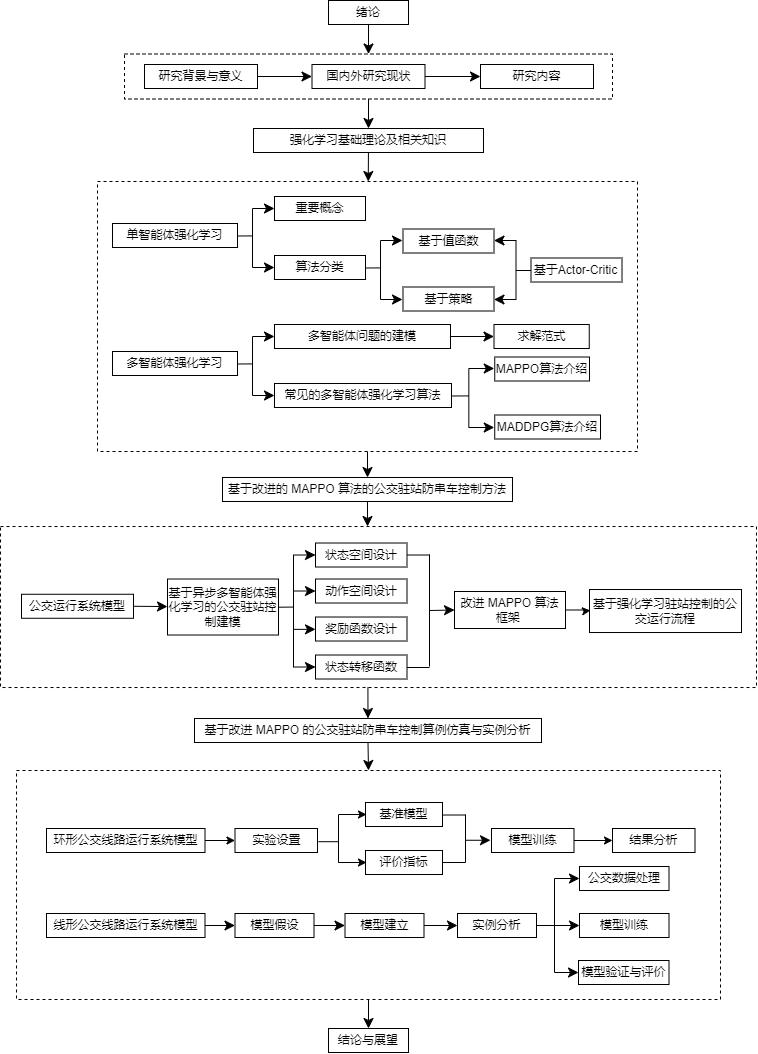
\includegraphics[width=1.0\linewidth]{figures/技术路线.png}
    \caption{技术路线}
    \label{fig:技术路线}
\end{figure}



\chapter{强化学习基础理论及相关知识}\label{第2章}
\section{单智能体强化学习基本原理}
强化学习（Reinforcement learning, RL）属于机器学习的一个分支。除强化学习外，机器学习
还包括监督学习（Supervised Learning）和无监督学习（Unsupervised Learning）。
% 监督学习依赖标注数据进行模式匹配，通过误差反馈机制建立输入输出的确定性映射关系；
% 无监督学习则聚焦于挖掘无标签数据的内在关联，揭示隐藏的数据结构特征。相较之下，
% 强化学习构建了独特的试错学习框架：智能体通过与环境动态交互获得延迟性奖励信号，
% 而非直接的正确答案指导，其核心目标在于构建最大化累积奖励的最优决策策略。
% 这种基于价值导向的序列决策机制，使其在动态环境建模和长期效益优化方面展现出独特优势。
在监督学习过程中，依赖标注数据进行模式匹配，通过误差反馈机制建立输入输出的确定性映射关系；
无监督学习则聚焦于挖掘无标签数据的内在关联，揭示隐藏的数据结构特征。
相较之下，强化学习构建了独特的试错学习框架，智能体通过与环境动态交互获得延迟性奖励信号，
而非直接的正确答案指导，其核心目标在于构建最大化累积奖励的最优决策策略。
强化学习与无监督学习的区别在于，无监督学习目的在于学习数据之间的隐含结构，
而强化学习通过基于价值导向的序列决策机制，在动态环境建模和长期效益优化方面展现出独特优势。

强化学习系统可以分为智能体（agent）和环境（environment）两部分，如下图\ref{fig:智能体与环境交互}所示。
智能体是强化学习系统中的决策者（决策做什么动作）和学习者（改变决定动作的策略），是主观可以控制的部分，
一个强化学习系统中可以有一个或多个智能体。
环境是与智能体交互的对象，除智能体外的所有东西，是客观不能改变的东西。
在强化学习过程中，智能体通过与环境交互，观察环境，根据观测信息做出动作（action），能够获得环境的
反馈信息，即奖励信号（reward），通过奖励信号来学习策略函数或价值函数，学习如何获取最大的奖励或者
付出最小化代价。
\begin{figure}[!ht]
    \centering
    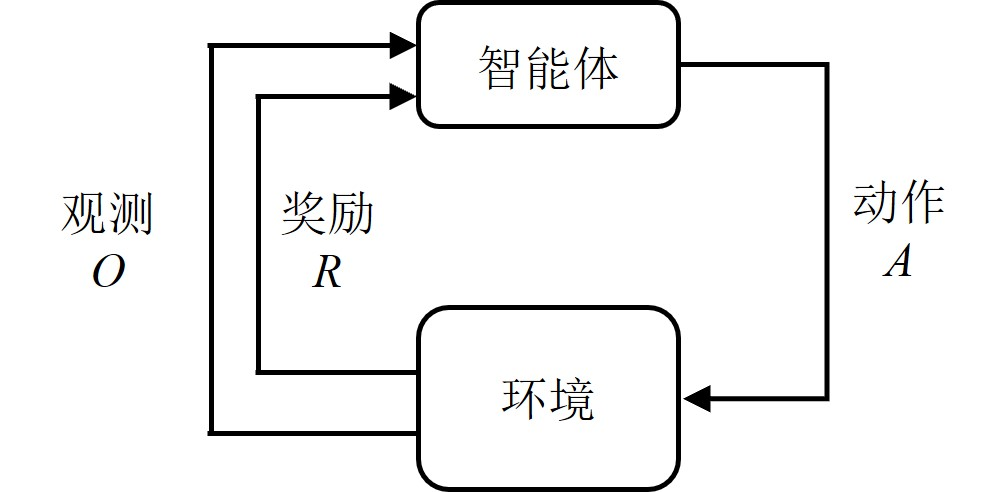
\includegraphics[width=0.5\linewidth]{figures/智能体与环境交互.jpg}
    \caption{智能体与环境交互}
    \label{fig:智能体与环境交互}
\end{figure}
\subsection{强化学习重要概念}
强化学习的理论框架主要由马尔可夫决策过程（Markov Decision Process, MDP）及其关键要素
构成\cite{lu2009similarity}。
该框架包含三个核心组成部分：智能体（Agent）、环境（Environment）以及二者间的动态交互机制。
在数学建模层面，状态空间与动作空间定义了系统的基本维度，状态转移函数和即时回报函数则表征
系统的动态特性与即时反馈机制。为实现长期收益最大化引入折扣系数对累积回报进行时间加权，
并通过价值函数和策略函数这两个核心分析工具来评估状态优劣和决策优化方向。
% 基础知识包括众多概念和模型，如马尔可夫决策过程（MDP）、智能体、环境、状态空间、动作空间、状态转移函数、即时回报函数、
% 累积回报、折扣系数、价值函数和策略函数等

（1）马尔可夫决策过程

马尔可夫决策过程（Markov Decision Process, MDP）作为强化学习的核心建模框架，可以用五元组
$( \mathcal{S},\mathcal{A},\mathcal{P},\mathcal{R},\gamma) $表示,其中：

$\mathcal{S}$：状态集合。

$\mathcal{A}$：动作集合。

$\mathcal{P}:\mathcal{S} \times \mathcal{A} \mapsto \mathcal{S}$表示状态转移函数，
$\mathsf{P} ( s_{\text{t}},a_{\text{t}},s_{\text{t+1}}) $
表示智能体执行动作$a_{\text{t}}$后状态$s_{\text{t}}$转移到状态$s_{\text{t+1}}$的概率。

$\mathcal{R}:\mathcal{S}\times \mathcal{A}\mapsto \mathcal{R}$是即时回报函数，
$\mathsf{R}  ( s_{\text{t}},a_{\text{t}},s_{\text{t+1}}) \in \mathcal{R}$
量化动作$a_{\text{t}}$执行后的单步收益（奖励）。

$\gamma \in  [ 0,1] $是折扣系数。

马尔可夫决策过程核心假设为马尔可夫性质（Markov Property），
该性质指，对于一个随机过程，给定当前的时刻的状态和过去所有时刻的状态，
未来的状态与过去的状态是相互独立的，表明未来状态的条件概率分布仅依赖于
现在的状态。数学表示如式（\ref{式1}）：
\begin{equation}\label{式1}
    \mathsf{P}(s_{t+1}| s_{0},s_{1},...,s_{t}) = \mathsf{P}(s_{t+1}| s_{t}).
\end{equation}

（2）即时回报函数

在强化学习中，即时回报函数是智能体学习的关键信息，智能体不知道输出动作的真实优劣，只能得到动作的
即时回报（即时奖励），智能体的目标函数是最大化与环境多次交互过程中的累积即时回报，一般称为
累积回报，即：
\begin{equation}\label{式2}
    \mathsf{G} = \sum_{t = 0}^{T}\mathsf{R}_{t}.   
\end{equation}

（3）累积折扣回报

在强化学习的决策优化框架中，目标是最大化长期奖励，对于连续的任务，
为避免无限时域下简单累加奖励造成未来奖励的总和趋于无穷大，引入了折扣因子$\gamma \in  [ 0,1] $，进而定义了累积折扣回报：
\begin{equation}\label{式3}
    \mathsf{G} = \sum_{t = 0}^{T}\gamma ^{t}\mathsf{R}_{t},   
\end{equation}
智能体通过时间偏好机制平衡即时与远期收益，该机制由折扣因子$\gamma$实现，若$\gamma = 0$，视为短视决策模型，
仅优化单步收益，完全忽视远期利益，若$\gamma = 1$，对于智能体来说当前的利益与远期的利益是同样重要的。

（4）策略函数

在智能体与环境的交互过程中，策略函数$\pi $作为智能体的决策核心，将环境状态$s$映射为可执行动作$a$，
表现为智能体根据观察到的环境状态$s$作出动作$a$。
策略函数根据策略的决策特性，可分为两类：

确定性策略，通过显式映射关系直接生成确定性动作，追求当前最优动作，表示为下式（\ref{式4}）:
\begin{equation}\label{式4}
    a = \pi (s ).   
\end{equation}

随机性策略：输出动作空间上的概率分布，决策过程具有随机性，通过概率采样平衡短期收益与长期信息获取，
表示为下式（\ref{式5}）：
\begin{equation}\label{式5}
    a \thicksim  \pi (s,a).
\end{equation}

（5）状态价值函数

状态价值函数是衡量智能体在状态$s$下，选择动作$a$能获得的期望累积奖励回报，状态价值越高的状态对于智能体越有
吸引力，在与环境的交互过程中，智能体会跳转到更高价值的状态，以获得更高的累积回报，在累积回报$G_{t}$
基础上，状态价值函数定义为：
\begin{equation}\label{式6}
    V_{\pi }( s) = E_{\pi}[ G_{t}| S_{t}=s], 
\end{equation}
$E[x]$表示期望，智能体基于策略函数$\pi$输出动作，获得即时回报$R_{t}$，若马尔可夫决策过程的决策总步数为$T$，
状态价值函数可定义为：
\begin{equation}\label{式7}
    V_{\pi }( s) = E_{\pi}[ \sum_{t = 0}^{T} \gamma ^tR_{t} | S_{t}=s]. 
\end{equation}

（6）动作价值函数

% 智能体期望能够基于策略函数获得最大的累积回报，
强化学习的核心目标在于构建能够最大化长期回报的策略函数，这一过程通过动作价值函数实现量化评估。
动作价值函数$Q(s,a)$定义为在策略$\pi$下，从状态$s$执行动作$a$后所获期望累积回报的数学期望
即：
\begin{equation}\label{式8}
    Q_{\pi }( s,a) = E_{\pi}[ G_{t} | S_{t}=s,A_{t}=a] = E_{\pi}[\sum_{t = 0}^{T} \gamma ^tR_{t} | S_{t}=s,A_{t}=a].
\end{equation}

通过该函数可建立策略优化的直接联系：最优策略$\pi^*(s)$始终选择当前状态下具有最大
Q值的动作，即：
\begin{equation}\label{式9}
    \pi^*(s) = \underset{a}{\arg\max}Q_{\pi }( s,a).
\end{equation}

（7）时序差分学习

时序差分学习（Temporal-Difference Learning, TD learning）采用自举（Bootstrapping）方法，用估计值来
估计并更新自身的数值，不需要采样完整的轨迹数据，只需要采样轨迹中智能体一步样本数据就可以更新状态价值，
从而提高状态价值函数$V_{\pi }( s)$的学习效率。采用时序差分学习方法的状态价值函数更新公式表示如下：
\begin{equation}\label{式10}
    V_{\pi }( s) =  E_{\pi}[R_{t} + \gamma V_{\pi }( S_{t+1}) | S_{t}=s],
\end{equation}
但是，因为策略$\pi $随着状态价值函数的更新一直变化，因此时序差分法估计出来的状态价值函数不一定是无偏估计。

同样的，采用时序差分学习方法估计的动作价值函数表示如下：
\begin{equation}\label{式11}
    Q_{\pi }( s,a) =  E_{\pi}[R_{t} + \gamma Q_{\pi }( S_{t+1}) | S_{t}=s,A_{t}=a].
\end{equation}
\subsection{强化学习算法分类}

强化学习算法按建模视角可以分为基于价值函数（value based）、基于策略梯度（policy based）和
演员-评论员（actor-critic）三类：



（1）基于价值函数（value based）的强化学习
通过构建状态价值函数$V(s)$或动作价值函数$Q(s,a)$
来量化长期奖励预期，决策时选择价值最大的动作。
基于价值函数的强化学习方法包括：Q-Learning算法\cite{watkins1992q}、深度Q网络（Deep Q-Network, DQN）算法\cite{mnih2015human}、
DQN的改进算法Double DQN\cite{van2016deep}和Dueling DQN\cite{wang2016dueling}等。
下面对经典的Q-Learning和DQN算法进行简单介绍。

\begin{itemize}
    \item Q-learning算法
\end{itemize}

Q-learning算法是一种无模型（Model-Free）异策略（off-policy）强化学习方法，
学习过程使用了时序差分法，能够进行离线学习，智能体在特定状态下
尝试执行一个动作，根据执行动作后获得的即时奖励或惩罚以及它所处状态的价值估计评估结果
的好坏。它不依赖于环境的具体模型，而是通过不断与环境交互，
逐步学习到每个状态-动作对的价值。
它通过学习一个动作价值函数（Q函数）来确定在每个状态下采取什么动作可以
获得最大的累积奖励，动作价值函数更新方式，如式(\ref{式12})：
\begin{equation}\label{式12}
    Q( s_{t},a_{t}) \leftarrow Q( s_{t},a_{t}) + \alpha [ R_{t}+\gamma\underset{a}{\max}Q( s_{t+1},a) - Q( s_{t},a_{t})],
\end{equation}
其中，$s_{t} $表示在时间步$ t$的状态，$a_{t}$表示在时间步$t$采取的动作，
$ R_{t}$表示在时间步$t$采取动作$a_{t}$后从环境中获得的即时奖励，
$\alpha \in (0,1]$为学习率，它控制了新的经验对旧的Q值更新的影响程度，
$\alpha$ 值越大，新经验的影响越大；$\alpha$越小，旧的Q值越不容易被改变。
$\gamma \in [0,1]$是折扣因子，调节远期奖励衰减速率，
$\gamma$ 越接近1，智能体越侧重远期收益；$\gamma$ 越接近0，智能体越注重即时奖励。
$\underset{a}{\max}Q( s_{t+1},a) $表示在下一步状态$s_{t+1}$下
所有可能动作中最大的 Q 值。

Q-Learning算法通常采用$ \epsilon$-贪心策略来进行动作的选择，
以概率$1- \epsilon $选择当前最优动作：$\underset{a}{\arg\max}Q( s_{t},a) $,
以概率$\epsilon$随机探索非最优动作，避免陷入局部最优。
通过动态调整$\epsilon$，实现早期充分探索与后期稳定利用的平衡。

\begin{itemize}
    \item 深度Q网络（Deep Q-Network, DQN）
\end{itemize}

DQN算法通过融合深度神经网络与Q-learning框架，
解决了传统表格方法在高维状态空间中的维度灾难问题。
% 传统的Q-learning是基于表格的算法，用于存储状态-动作对所对应的Q值。
% 但是在实际应用场景中，状态空间往往极其庞大或者是连续的，这就使得使用表格来存
% 储所有的Q值变得不切实际。
% DQN则借助深度神经网络来近似表示Q函数，即$Q(s,a;\theta )$，
其核心创新在于用神经网络参数化Q函数$Q(s,a;\theta)$，$\theta $是神经网络的参数。
通过不断地与环境进行交互，并对参数进行更新，使得该网络能够精准地估计出在不同状态下执行不
同动作所对应的Q值。

DQN算法的网络架构包含两个网络：在线网络（Online Network）和目标网络（Target Network）。
在线网络（Online Network）实时生成Q值估计，参数$\theta $通过梯度下降更新：
\begin{equation}\label{式13}
    Q(s, a) = E \left[ \sum_{t = 0}^{\infty} \gamma^{t} r_{t} \mid s_{0} = s, a_{0} = a \right],
\end{equation}
其中，$\gamma\in [0,1]  $是折扣因子，控制远期奖励衰减速率。
目标网络（Target Network）提供稳定的Q值目标，与在线网络（Online Network）结构一致，
但参数$ \theta'$更新的频率较低，目标网络的Q值计算公式如下式（\ref{式14}）:
\begin{equation}\label{式14}
    y_{j} = 
    \begin{cases}
    r_{j} & \text{若在步骤 } j + 1 \text{ 时，episode结束}\\
    r_{j} + \gamma \max_{a'} Q'(s_{j + 1}, a'; \theta') & \text{否则}
    \end{cases}
\end{equation}
其中，$r_{j}$是智能体在状态$s_j $下采取动作$ a_j$后所获得的奖励。
$Q'(s_{j + 1}, a'; \theta') $是目标网络对状态$s_{j + 1} $下动作$ a' $的 Q 值估计，
$\theta' $是目标网络的参数。

通过最小化估计Q值与目标Q值的均方误差（MSE）实现参数更新：
\begin{equation}\label{式15}
    L(\theta) = E \left[ \left( Q(s, a; \theta) - y \right)^2 \right],
\end{equation}
其中，$ Q(s, a; \theta)$ 是在线网络对状态$s$下采取动作$a$时的 Q 值估计，
$y$则是与之对应的目标Q值。通常会使用随机梯度下降（SGD）算法或者其改进版本（如Adam优化器）来最
小化损失函数，进而实现对在线网络参数$\theta$ 的更新，见下式：
\begin{equation}\label{式16}
    \theta \leftarrow \theta - \alpha \nabla_{\theta} L(\theta),
\end{equation}
其中，$\alpha $ 代表学习率，它决定了每次参数更新的步长大小。$\nabla_{\theta} L(\theta) $表示损失函数
关于参数$ \theta$的梯度。

DQN通过经验回放（Experience Replay）进行数据存储和批量采样，
具体来说，就是将智能体在与环境交互过程中所产生的经验元组存储到经验回放缓冲区。
在进行训练时，会从这个缓冲区中随机抽取一批经验样本，打破时序相关性，减少方差，以此来对网络参数进行更新。
这种机制能够提升数据利用率，缓解非平稳分布问题。

% （2）基于策略的强化学习算法

（2）基于策略梯度（policy based）的强化学习算法直接参数化策略函数
$\pi_{\theta}(a|s)$，通过梯度上升优化策略参数$θ$，适用于连续动作空间场景，典型代表
策略梯度（Policy Gradient）算法\cite{sutton1999policy}。

\begin{itemize}
    \item 策略梯度算法（Policy Gradient）
\end{itemize}

该方法摒弃了传统价值函数估计的间接优化路径，转而直接参数化策略函数
$\pi_{\theta}(a|s)$，通过梯度上升对参数$\theta$进行端到端优化。
相较于基于价值函数的算法，其核心优势在于直接策略搜索能力。
策略函数$\pi_{\theta}(a|s)$将状态$s$映射到动作$a$的概率分布，直接生成动作决策。
优化目标是最大化轨迹$\tau = (s_0, a_0, r_0, s_1, a_1, r_1, \cdots, s_T, a_T, r_T)$ 
的期望累积奖励，其目标函数如下式（\ref{式2-1}）所示。
\begin{equation}\label{式2-1}
    J(\theta) = E_{\tau \sim \pi_{\theta}} \left[ \sum_{t = 0}^{T} \gamma ^ t r(s_t, a_t) \right],
\end{equation}
其中，$\gamma $ 为折扣因子，$\tau = (s_0, a_0, r_0, s_1, a_1, r_1, \cdots, s_T, a_T, r_T)$ 
表示一个轨迹（trajectory），即智能体在环境中从初始状态开始，
经过一系列状态和动作，直到终止状态的完整序列。

算法会根据智能体在环境中的经验，估计策略参数$\theta$的梯度，
策略梯度定理（Policy Gradient Theorem）
给出了目标函数$J(\theta)$关于策略参数$\theta$的梯度的计算公式,见下式（\ref{式2-2}）：
\begin{equation}\label{式2-2}
    \nabla_{\theta} J(\theta) = E_{\tau \sim \pi_{\theta}} \left[ \sum_{t = 0}^{T} \nabla_{\theta} \log \pi_{\theta}(a_t|s_t)\cdot  G_t \right],
\end{equation}
其中，$\nabla_{\theta} \log \pi_{\theta}(a_t|s_t)$ 
是策略函数 $\pi_{\theta}(a|s)$ 在状态 $s_t$ 采取动作 $a_t$ 的对数概率关于参数
$\theta$ 的梯度；
$G_t = \sum _{k=t}^T \gamma ^{k-t}r_k$ 为累积回报。 

采用梯度上升来更新策略参数$\theta$，更新方向如下式（\ref{式2-3}）：
\begin{equation}\label{式2-3}
    \theta \leftarrow \theta + \alpha \nabla_{\theta} J(\theta),
\end{equation}
其中 $\alpha$ 是学习率，用来控制每次参数更新的步长，梯度方向为策略目标函数的最大化方向。


% （3）演员-评论员强化学习算法
（3）演员-评论员（Actor-Critic）强化学习算法同时利用了基于价值和基于策略的方法，算法框架如下
\ref{fig:Actor-Critic算法框架}图所示。
基于Actor-Critic的算法包括：优势演员-评论员算法（Advantage Actor-Critic, A2C）\cite{mnih2016asynchronous}、
异步优势演员-评论家算法（Asynchronous Advantage Actor-Critic, A3C）\cite{mnih2016asynchronous}、
Soft Actor-Critic算法（SAC）\cite{haarnoja1861soft}、
信赖域策略优化算法（Trust Region Policy Optimization, TRPO）\cite{schulman2015trust}、
确定性策略梯度算法（Deterministic Policy Gradient, DPG）\cite{silver2014deterministic}、
深度确定性策略梯度算法（Deep Deterministic Policy Gradient，DDPG）\cite{lillicrap2015continuous}、
近端策略优化算法（Proximal Policy Optimization, PPO）\cite{schulman2017proximal}等。
下面主要介绍PPO算法和DDPG算法。
\begin{figure}[!ht]
    \centering
    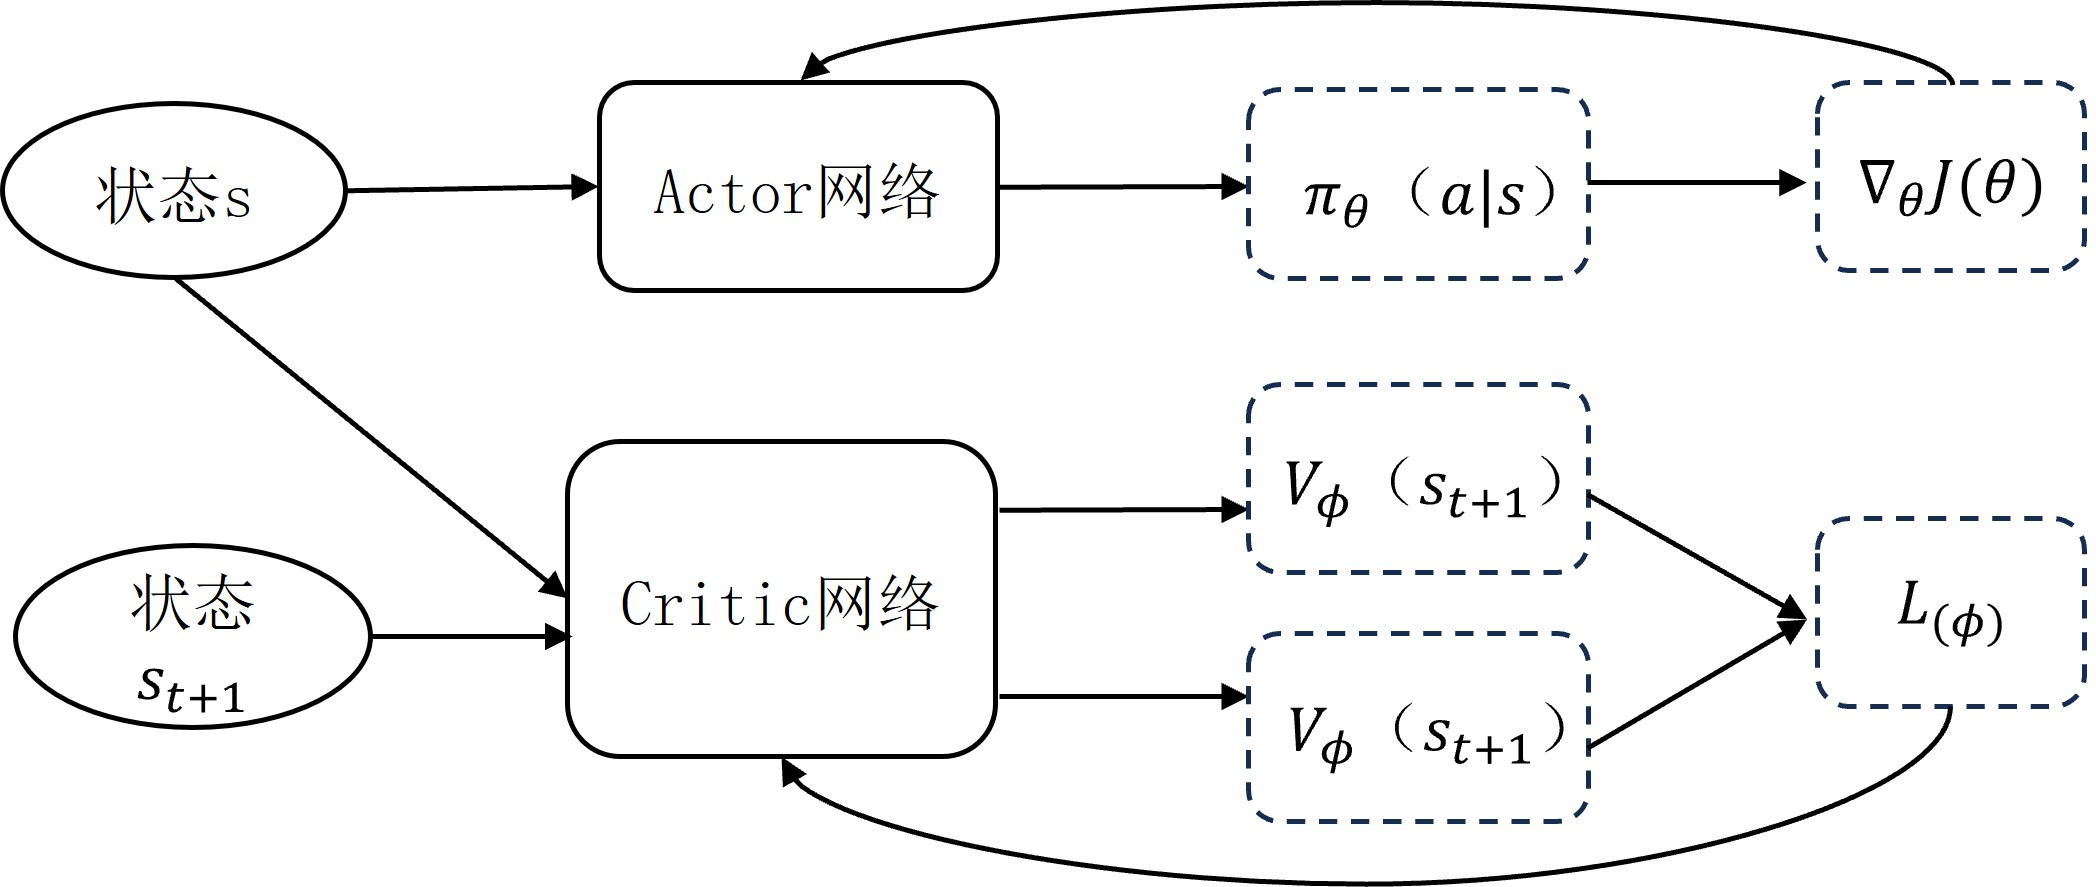
\includegraphics[width=0.7\linewidth]{figures/Actor-Critic算法框架.jpg}
    \caption{Actor-Critic算法框架}
    \label{fig:Actor-Critic算法框架}
\end{figure}

\begin{itemize}
    \item 深度确定性策略梯度（Deep Deterministic Policy Gradient, DDPG）算法
\end{itemize}

DDPG算法作为一种面向连续控制任务的无模型（Model-Free）强化学习算法，
通过演员-评论员（Actor-Critic）架构与确定性策略梯度（Deterministic Policy Gradient, DPG）
的结合，实现了高维动作空间下的高效策略优化。
采用双网络架构设计：策略网络（Actor）和价值网络（Critic）。
确定性策略函数$\mu(s;\theta^{\mu})$直接将状态映射为连续动作，
价值网络则评估该动作在当前状态下的价值$Q(s, a;\theta^{Q})$。

基于确定性策略梯度定理（Deterministic Policy Gradient Theorem），
策略网络（Actor）的参数更新方向由价值网络（Critic）对动作的梯度引导，
策略梯度的计算公式如下式（\ref{式20}）：
\begin{equation}\label{式20}
    \nabla_{\theta^{\mu}} J \approx E_{s_t \sim \mathcal{D}}\left[\nabla_{\theta^{\mu}} \mu(s_t;\theta^{\mu}) \nabla_{a} Q(s, a;\theta^{Q})\big|_{s = s_t, a = \mu(s_t;\theta^{\mu})}\right],
\end{equation}
其中，$\theta^{\mu}$ 是策略网络（Actor）的参数，$\theta^{Q}$ 是价值网络（Critic）的参数，
$Q(s, a;\theta^{Q})$ 是价值网络（Critic）对状态-动作对的价值估计，
$\mathcal{D}$ 是经验回放缓冲区。
通过计算Actor对参数的梯度和Critic对动作的梯度的乘积，指导Actor参数向提升Q值的方向更新。


价值网络（Critic）的目标是最小化估计值和目标值之间的均方误差。损失函数的计算公式见式（\ref{式21}）：
\begin{equation}\label{式21}
    L(\theta^{Q}) = E_{(s_t, a_t, r_t, s_{t + 1}) \sim \mathcal{D}}\left[\left(Q(s_t, a_t;\theta^{Q}) - y_t\right)^2\right],
\end{equation}
其中，目标值 $y_t$ 的计算方式为下式：
\begin{equation}\label{式22}
    y_t = r_t + \gamma Q'(s_{t + 1}, \mu'(s_{t + 1};\theta^{\mu'});\theta^{Q'}),
\end{equation}
$r_t$ 是在状态 $s_t$ 采取动作 $a_t$ 后获得的即时奖励；
$\gamma$ 是折扣因子，用于平衡即时奖励和未来奖励的重要性；
$Q'$ 和 $\mu'$ 分别是目标价值网络和目标策略网络，他们的参数$\theta^{Q'}$ 和 $\theta^{\mu'}$
分别通过软更新同步，二者更新过程相互独立，确保目标网络参数缓慢跟踪在线网络，以保证训练的稳定性，
更新公式见下
式（\ref{式23}）和（\ref{式24}）：
\begin{equation}\label{式23}
    \theta^{Q'} \leftarrow \tau \theta^{Q} + (1 - \tau) \theta^{Q'}, 
\end{equation}
\begin{equation}\label{式24}
    \theta^{\mu'} \leftarrow \tau \theta^{\mu} + (1 - \tau) \theta^{\mu'},
\end{equation}
其中，$\tau$ 是一个较小的超参数，通常取一个很小的值，
确保目标网络参数更新缓慢，维持训练稳定性。

% （2）PPO算法

\begin{itemize}
    \item 近端策略优化算法（Proximal Policy Optimization, PPO）
\end{itemize}

传统策略梯度方法因策略更新幅度不可控，易导致训练崩溃或收敛缓慢。
近端策略优化算法（PPO）通过限制新旧策略差异，以近似满足信任域约束，显著提升了训练稳定性。
与其他算法相比，PPO 与其他算法相比，PPO 在稳定性、实现简单性和通用性上表现突出，成为深度强化学习的标杆算法之一。

PPO算法核心在于构建有界策略更新目标函数，其主流实现包括两种形式：近端策略优化裁剪（PPO-Clip）
和近端策略优化惩罚（PPO-Penalty）。

近端策略优化惩罚（PPO-Penalty）是通过在目标函数中添加一个KL散度惩罚项来限制策略更新的幅度。
目标函数定义如下式（\ref{式19}）：
\begin{equation}\label{式19}
    L^{KL - PEN}(\theta) = \hat{E}_t\left[r_t(\theta) \hat{A}_t - \beta \text{KL}\left[\pi_{\theta_{old}}(\cdot|s_t), \pi_{\theta}(\cdot|s_t)\right]\right],
\end{equation}
其中，$r_t(\theta)=\frac{\pi_{\theta}(a_t|s_t)}{\pi_{\theta_{old}}(a_t|s_t)}$是
新旧策略的概率比率；$ \beta $初始为固定值，但会根据实际 KL 散度与目标值的偏差动态调整：
若 KL 散度过大，则增大$\beta $以加强约束；若过小，则减小$\beta $以放松约束，以
平衡策略更新与稳定性；
$KL \left[\pi_{\theta_{old}}(\cdot|s_t), \pi_{\theta}(\cdot|s_t)\right]$
表示旧策略到新策略的 KL 散度，衡量两者差异。

近端策略优化裁剪（PPO-Clip）更常用，因其省去了动态调整KL惩罚系数的复杂性，
通过引入裁剪函数来限制策略更新的幅度。目标函数定义如下式（\ref{式18}），后
文无特别说明，提到的PPO算法均采用PPO-Clip。
\begin{equation}\label{式18}
    L^{CLIP}(\theta) = \hat{E}_t\left[\min\{ r_t(\theta) \hat{A}_t, \text{clip}(r_t(\theta), 1 - \epsilon, 1 + \epsilon) \hat{A}_t\} \right],
\end{equation}
其中，$r_t(\theta)=\frac{\pi_{\theta}(a_t|s_t)}{\pi_{\theta_{old}}(a_t|s_t)}$是
新旧策略下动作概率的比值，
$\theta_{old} $是更新前的策略参数，$ \epsilon$是一个超参数，
用于控制裁剪的范围。
裁剪函数$\text{clip}(r_t(\theta), 1 - \epsilon, 1 + \epsilon)$将 
$r_t(\theta)$限制在$[1 - \epsilon, 1 + \epsilon]$范围内。
% 该目标函数的作用机制是，当$ \hat{A}_t > 0$（动作优于平均水平），
% 限制$r_t(\theta) \leq 1 + \epsilon$，防止策略过度提升该动作的概率；
% 当$ \hat{A}_t < 0$（动作劣于平均水平），
% 限制$r_t(\theta) \geq  1 - \epsilon$，防止策略过度降低该动作的概率。


PPO-Clip通过分段函数
限制策略更新的幅度，示意图如下图\ref{fig:PPO-Clip示意图}所示：
\begin{itemize}
    \item $ \hat{A}_t > 0$（图a）：动作优于平均水平，限制$r_t(\theta) \leq 1 + \epsilon$，防止策略过度提升该动作的概率；
    \item $ \hat{A}_t < 0$（图b）：动作劣于平均水平，限制$r_t(\theta) \geq  1 - \epsilon$，防止策略过度降低该动作的概率。
\end{itemize}

\captionsetup{justification=centering} % 设置题注内容居中
\begin{figure}[!ht] 
    \centering
    \begin{subfigure}[b]{0.47\textwidth}
        \centering
        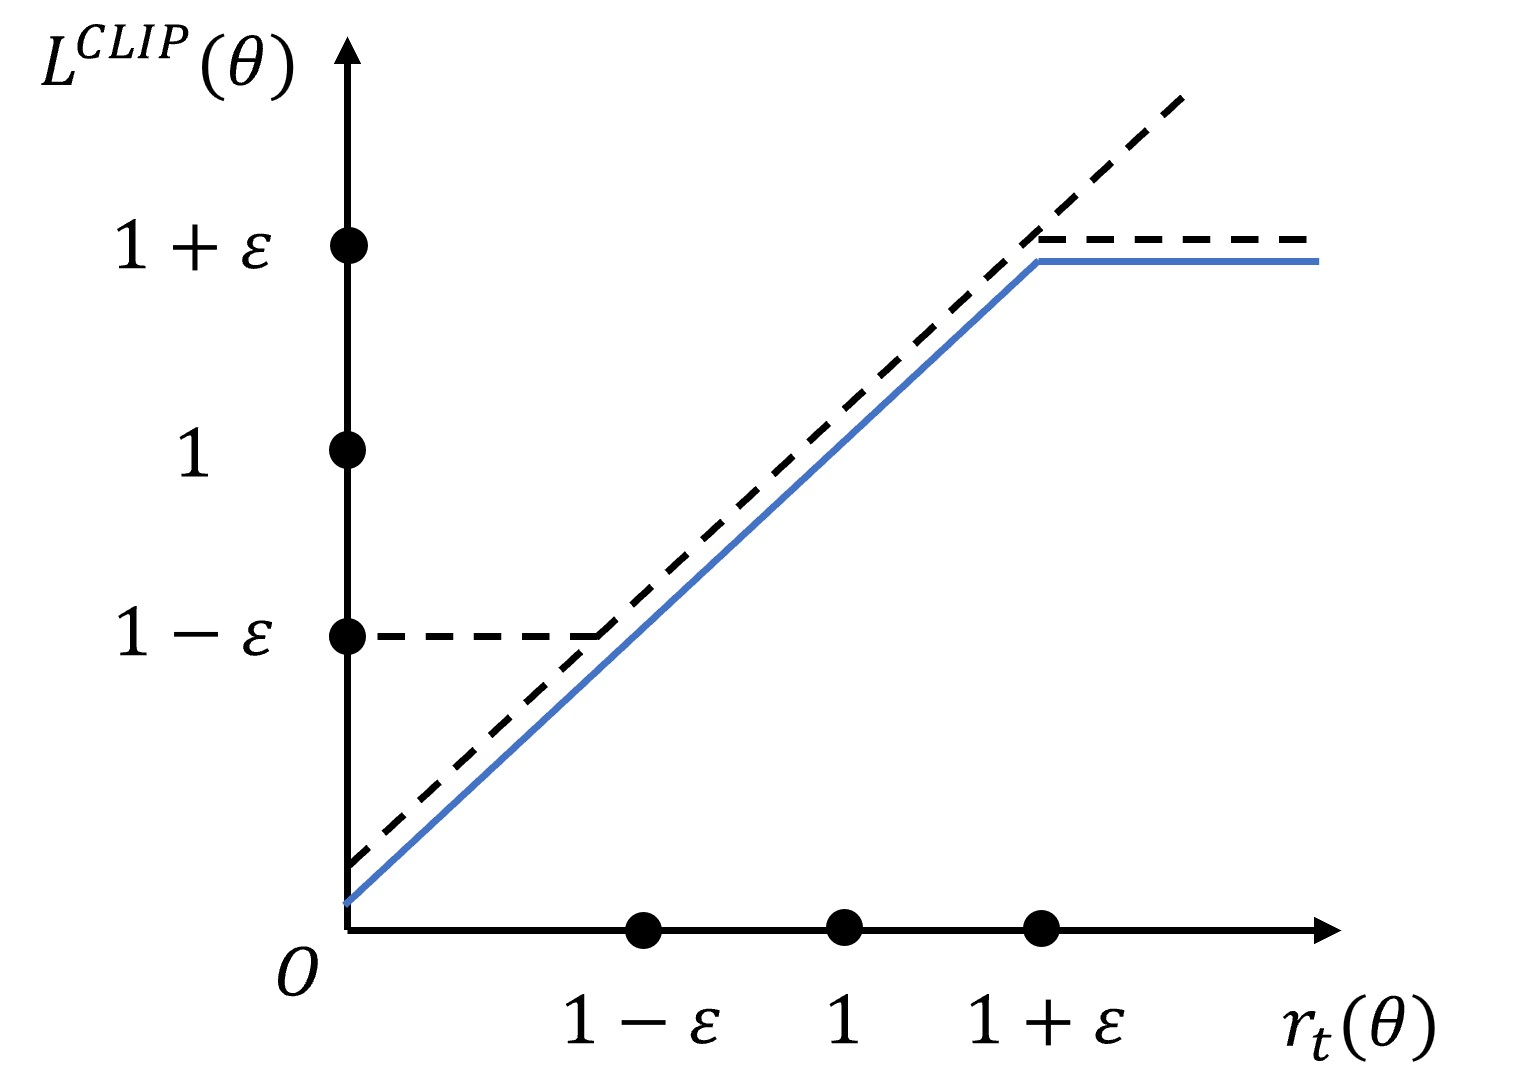
\includegraphics[width=\linewidth]{figures/剪切函数大于0.jpg}
        \caption{$\hat{A}_t > 0$}
    \end{subfigure}
    \quad
    \begin{subfigure}[b]{0.47\textwidth}
        \centering
        
\includegraphics[width=\linewidth]{figures/剪切函数小于0.png.jpg}
        \caption{$\hat{A}_t < 0$}
    \end{subfigure}
    \caption{PPO-Clip示意图}
    \label{fig:PPO-Clip示意图}
\end{figure}
通过这一设计，PPO-Clip 在避免策略更新过大的同时，无需动态调整超参数（如 PPO-Penalty 中的 
$ \beta $），显著简化了实现流程。

基于策略梯度定理，策略参数$\theta$的更新方向由优势函数加权的策略对数梯度决定，以最大化期望回报。
其梯度表达式为:
\begin{equation}\label{式17}
    \nabla_{\theta} L^{CLIP}(\theta) = \hat{E}_t\left[\nabla_{\theta} \log \pi_{\theta}(a_t|s_t) \hat{A}_t\right],
\end{equation}
其中， $\pi_{\theta}(a_t|s_t)$ 是策略网络在状态$s_t $下采取动作$a_t$的概率；
$ \hat{A}_t$是优势函数的估计值，通常通过广义优势估计（Generalized Advantage Estimation, GAE）或其他方法近似计算，表示动作$a_t$相对于状态$s_t$下平均水平的优势；
$\hat{E}_t$表示基于采样数据的经验期望。

\section{多智能体强化学习基本原理}

多智能体强化学习（Multi-Agent Reinforcement Learning, MARL）
通过研究多个智能体在共享环境中的协同决策问题，扩展了传统单智能体强化学习的理论框架。
如下图\ref{fig:多智能体强化学习环境概览}所示。
每个智能体基于局部观测独立决策，同时环境状态受所有智能体联合动作影响，形成动态交互网络。
其核心挑战：一是环境的非平稳性，智能体并行学习导致环境动态持续变化，
联合动作空间下状态转移的概率$\mathcal{P}(s^{'}|s,a_i,a_{-i})$依赖其他智能体的
联合动作$a_{-i} $；
二是联合状态空间$\mathcal{S}$和动作空间$\mathcal{A}$随着智能体数量的增加呈指数增长，
可能会导致维度爆炸。
\begin{figure}[!ht]
    \centering
    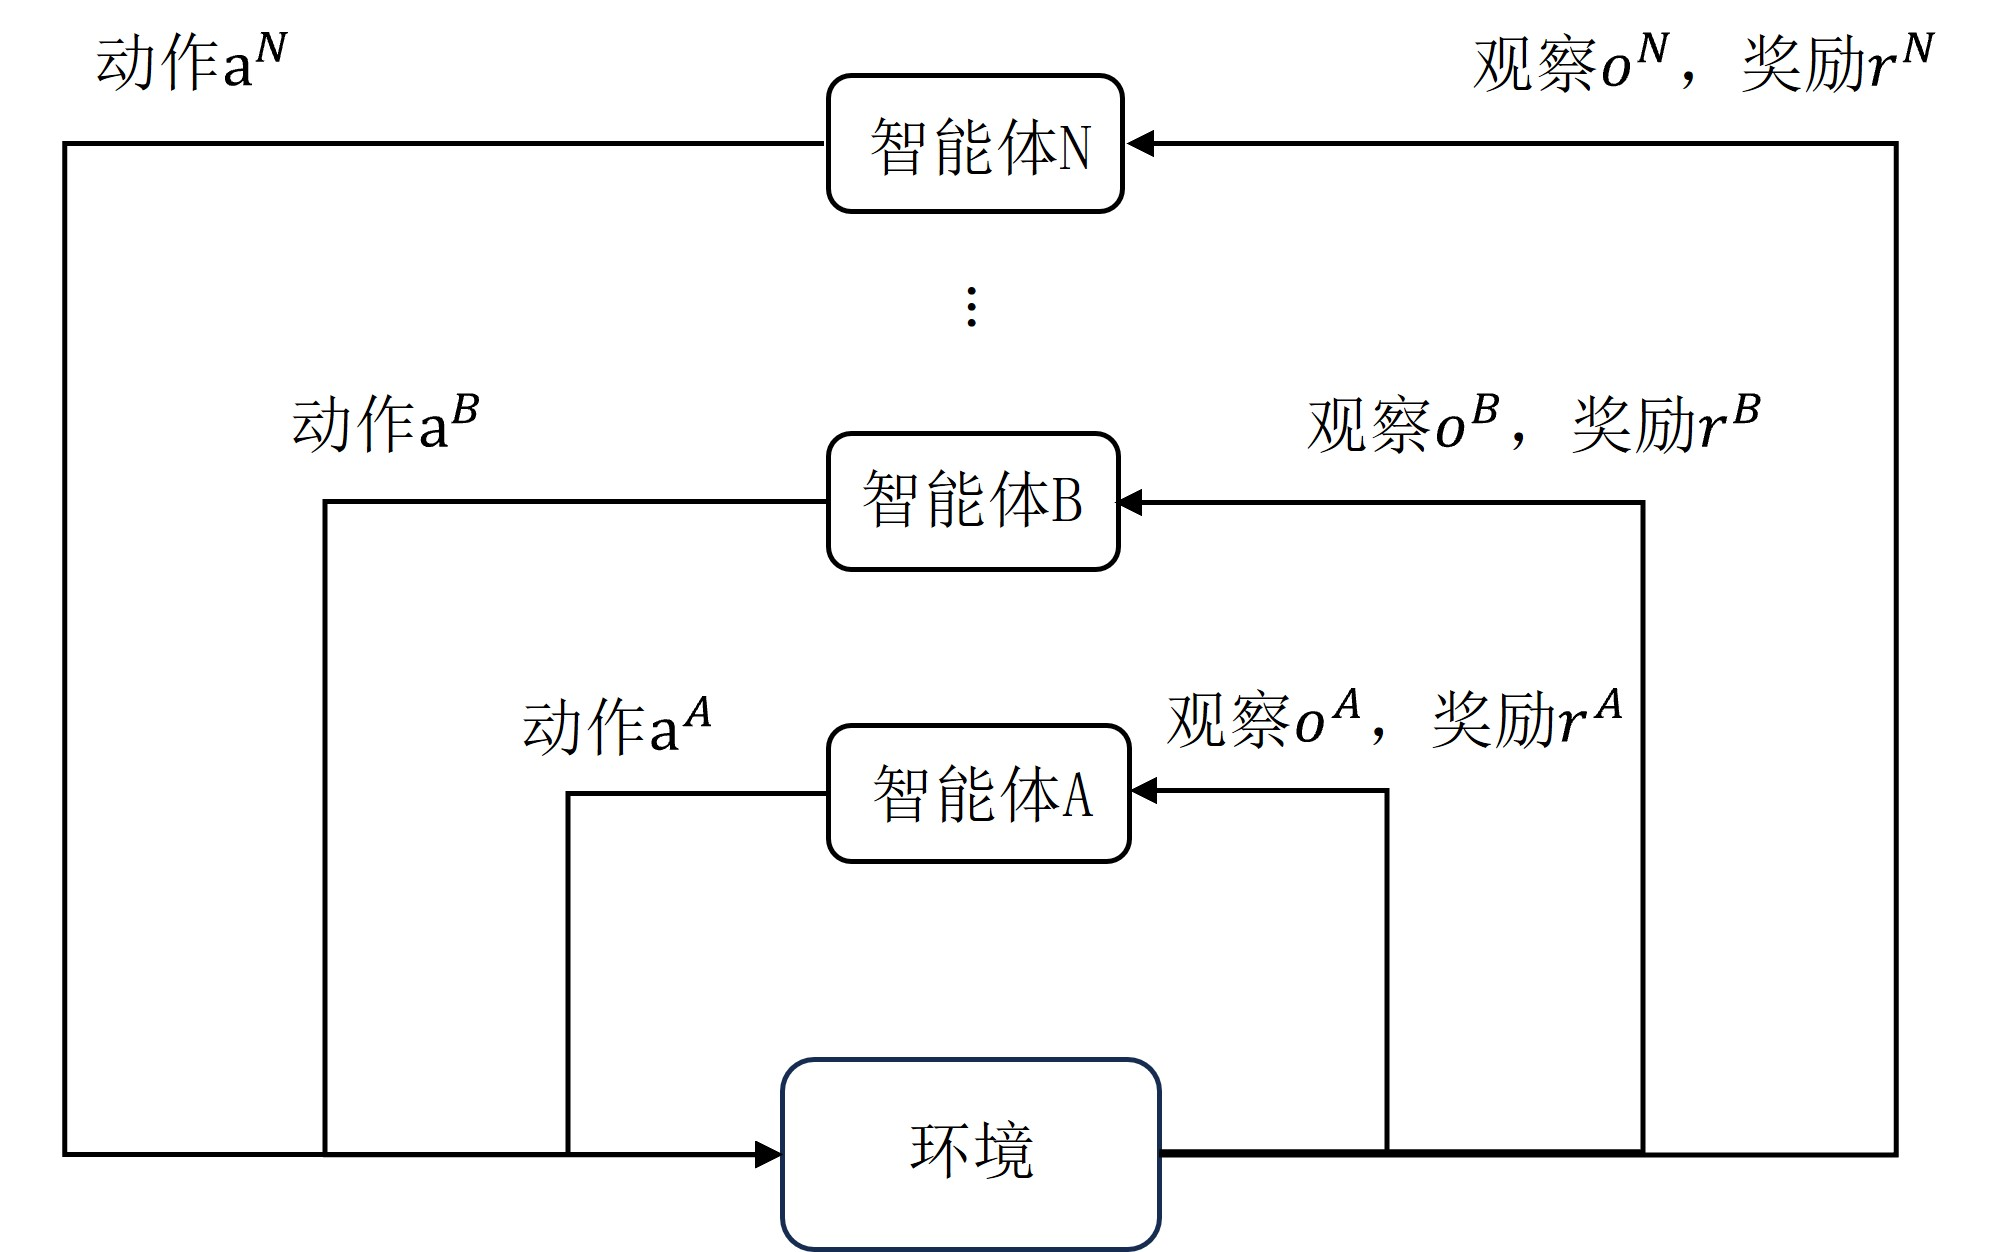
\includegraphics[width=0.75\linewidth]{figures/多智能体强化学习环境概览.jpg}
    \caption{多智能体强化学习环境概览}
    \label{fig:多智能体强化学习环境概览}
\end{figure}
\subsection{多智能体问题的建模}
马尔可夫决策过程扩展到多智能体强化学习被定义为马尔可夫博弈（Markov Game, MG）。
多智能体强化学习问题可形式化为马尔可夫博弈（Markov Game, MG），可以用一个
元组来表示，见下式（\ref{式25}）：
\begin{equation}\label{式25}
    G =  (N,\mathcal{S},\mathcal{A},\mathcal{P},\mathcal{R},\gamma),
\end{equation}

其中：

$N$ —— 智能体的数目；

$\mathcal{S} = \{ S_{1}, S_{2} , \cdots ,S_{N}\} $ —— 所有智能体的状态集合；

$\mathcal{A} =\{ A_{1},  A_{2} , \cdots , A_{N}\} $ —— 所有智能体的动作集合；

$\mathcal{P}:\mathcal{S} \times \mathcal{A} \mapsto \mathcal{S}$ —— 状态转移函数；

$\mathcal{R} = \{ R_{1} , R_{2} ,  \cdots ,R_{N}\} $ —— 所有智能体奖励函数的集合，
每个$R_{i}$由当前状态和所有智能体的动作决定：$\mathcal{S}\times A_{1},\cdots ,\times A_{N} \mapsto  R_{i}$；

$\gamma \in  [ 0,1] $ —— 折扣系数。

选择动作的策略由条件概率给出$\pi _{\theta_{i} }=P( A_{i}| O_{i}) $，
其中$O_{i}$是智能体$i$对当前状态$\mathcal{S}$的观察。

\subsection{多智能体强化学习的求解范式}
多智能体强化学习的基本求解范式可以分为完全中心化（Fully Centralized）方法、完全去中心化（Fully Decentralized）方法
和中心化训练去中心化执行（Centralized Training with Decentralized Execution，CTDE）三种。



（1）完全中心化（Fully Centralized）

完全中心化方法依赖中央控制器聚合全局信息，
把所有智能体的动作连起来作为一个联合动作，中央处理器学习一个统一的策略或价值函数，
统一进行决策，智能体仅按照中央控制器的指令执行动作，
所有智能体的策略更新都由中央控制器来完成，智能体不能独立学习。
这种方式能充分利用信息，学习效率高，所有智能体的状态和动作
是已知的，所以环境依旧是稳态的，能够找到理论上的最优联合策略，但通信开销极大，
随着智能体增多，中央控制器计算负担呈指数级增长，一旦中央控制器出现
故障，整个系统就会崩溃，同时也不能很好的扩展到智能体数量很多或者环境复杂的情况，容易导致
维度爆炸。

（2）完全去中心化（Fully Decentralized）

每个智能体独立学习策略不与其他智能体通信，视其他智能体为环境的动态部分。
这样的优点是通信开销几乎为零，扩展性强，可轻松扩展到大规模多智能体系统，
不会遇到维度灾难导致训练不能进行，部分智能体故障不会影响整体运行；
缺点是非稳态环境收敛困难，局部观测限制策略优化，且智能体间缺乏协调，行为易冲突，导致整体性能不佳。

（3）中心化训练去中心化执行（Centralized Training with Decentralized Execution, CTDE）

中心化训练去中心化执行（CETD）结合了前两者的优点，训练时，中央控制器可以获取全局状态信
息或多个智能体的联合信息，学习一个集中的价值函数或者其他用于指导策略学习的参数。
执行阶段每个智能体独立进行决策，不需要与中央控制器进行实时通信。
CTDE的优点是可以有效的利用全局信息提高学习效率，达到更稳定的训练效果，
同时可以平衡学习效率与执行效率，策略协调性增强；
缺点是训练阶段需全局通信，智能体与中央控制器之间进行大量的信息交互。

\subsection{多智能体强化学习算法分类}

基于智能体之间的关系可以将多智能体强化学习算法分为三类，如下表\ref{tab2-1}所示。




% （1）完全协作型算法


% 分为完全协作算法（如QMIX 算法）、
% 完全竞争算法（如Nash Q - learning）和混合关系算法三种。
% 完全协作的多智能体的目标是一致的，他们需要通过协作来最大化共同的奖励；
% 各个智能体的奖励函数通常是相同或者高度相关的，
% 一个智能体的成功往往依赖于其他智能体的行为。
% 完全竞争的智能体的目标是
% 相互冲突的，一个智能体的收益往往意味着其他智能体的损失；
% 混合的多智能体之间既有协作又有竞争，在
% 复杂环境中，智能体在某些任务上需要协作，在其他任务上存在竞争。

下面介绍两种常见的多智能体强化学习：
多智能体近端策略优化算法（Multi-Agent Proximal Policy Optimization, MAPPO）和
多智能体深度确定性策略梯度（Multi-Agent Deep Deterministic Policy Gradient, MADDPG）

\begin{table}[!h]
\centering
\caption{多智能体强化学习算法分类}
\label{tab2-1}
% \begin{tabular}{cp{0.8\textwidth}}
\begin{tabular}{>{\centering\arraybackslash}m{3cm} >{\raggedright\arraybackslash}m{5cm} >{\centering\arraybackslash}m{2cm} >{\raggedright\arraybackslash}m{3cm}}
\toprule
\textbf{算法类别}  & \multicolumn{1}{c}{\textbf{场景特征}} & \textbf{典型算法} & \multicolumn{1}{c}{\textbf{技术挑战}}\\
\midrule
完全协作型算法 & 共同目标：所有智能体共享奖励函数$R_1 = R_2 = ... =R_N$；\newline
强耦合决策：个体动作对团队收益产生链式影响 & QMIX、VDN & 信用分配（Credit Assignment）问题；\newline 非平稳性导致的策略震荡\\
完全竞争型算法 & 零和博弈：智能体收益满足$\sum_{i=1}^N R_i = 0$；\newline
纳什均衡求解：策略组合$\pi^* = (\pi_1*,...,\pi_N*)$ 满足单方面偏离无收益 & Nash Q-Learning
& 高维策略空间计算复杂度；\newline 均衡解的非唯一性问题  \\
混合关系型算法 & 动态角色切换：智能体在子任务中呈现协作/竞争行为；\newline
分层奖励结构：全局奖励$R_g$与个体奖励$R_i$共存 & MADDPG & 多目标优化权衡；动态关系建模\\
% 站点客流量 & 站点乘客数量的变化会影响公交车的停留时间，尤其是当某站点乘客数量激增时 \\
\bottomrule
\end{tabular}
\end{table}

（1）多智能体近端策略优化算法（Multi-Agent Proximal Policy Optimization, MAPPO）

MAPPO 作为PPO算法在多智能体场景的扩展，通过集中式训练与分布式执行（CTDE）
框架实现智能体间的协同策略优化。
在训练阶段，智能体的价值网络（Critic）能获取全局状态学习全局价值函数，使智能体在策略更新时隐式考量其他智能体的行为；
在执行阶段，每个智能体仅依据自身观测的局部状态选择动作，
维持系统分布式控制特性。

\begin{itemize}
    \item 策略更新：对于每个智能体\(i\)，其策略更新借助类似 PPO 的目标函数，
\end{itemize}
且策略仅依赖自身观测\(o_i\)，目标函数见下式（\ref{式2-6}）：
\begin{equation}\label{式2-6}
    L^{CLIP}_i(\theta_i) = E_t \left( \min \{  r_t(\theta_i) \hat{A}_t^i, \text{clip}(r_t(\theta_i), 1 - \epsilon, 1 + \epsilon) \hat{A}_t^i\}  \right),
\end{equation}
其中
$r_t(\theta_i) = \frac{\pi_{\theta_i}(a_t^i | o_t^i)}{\pi_{\theta_i^{\text{old}}}(a_t^i | o_t^i)} $
是智能体\(i\)的策略比率，优势函数\(\hat{A}_t^i\)基于广义优势估计
（GAE）计算，见下式（\ref{式2-8}）：
\begin{equation}\label{式2-8}
    \hat{A}_t^i = \sum_{k = 0}^{\infty}(\gamma\lambda)^k\delta_{t + k}^i,
\end{equation}
其中\(\delta_{t + k}^i\)是\(t + k\)时刻的 TD 误差，见下式（\ref{式2-9}）：
\begin{equation}\label{式2-9}
    \delta_{t+k}^i = r_{t+k}^i + \gamma V(s_{t+k+1}; \phi^{\text{old}}) - V(s_{t+k}; \phi^{\text{old}}).
\end{equation}

\begin{itemize}
    \item 价值函数估计：所有智能体共享Critic网络\(V(s; \phi)\)，基于全局状态估计价
\end{itemize}
值函数，损失函数为：
\begin{equation}\label{式2-7}
    L(\phi) = E_{s_t, s_{t+1}, r_t} \left( \left( V(s_t; \phi) - (r_t + \gamma V(s_{t+1}; \phi^{\text{old}})) \right)^2 \right).
\end{equation}

% \begin{itemize}
%     \item 价值函数估计：智能体\(i\)的价值函数\(V_i(s)\)由中心化的 Critic 网络估计，Critic
% \end{itemize}
% 网络利用全局状态\(s\)以及所有智能体动作\(a_1, a_2, \cdots, a_N\)
% 估计全局价值函数，其目标是最小化均方误差（MSE）损失函数，见下式（\ref{式2-7}）：
% \begin{equation}\label{式2-7}
%     L(\phi_i) = E_{s_t, r_t, s_{t + 1}} \left( \left( V_i(s_t; \phi_i) - R_t \right)^2 \right)
% \end{equation}

（2）多智能体深度确定性策略梯度（Multi-Agent Deep Deterministic Policy Gradient, MADDPG）

MADDPG是从单智能体的深度确定性策略梯度（Deep Deterministic Policy Gradient, DDPG）
算法扩展而来，采用集中式训练与分布式执行（CTDE）。
每个智能体独立维护策略网络（Actor）和价值网络（Critic），
训练时Critic利用全局状态和所有智能体动作，执行时Actor仅依赖局部观测。

\begin{itemize}
    \item 策略网络更新
\end{itemize}

智能体\(i\)的策略梯度为：
\begin{equation}\label{式2-10}
    \nabla_{\theta^{\mu_i}} J \approx \frac{1}{B} \sum_{j=1}^B \nabla_{a_i} Q_{\theta^Q_i}\left(s^j, \mu_1(o_1^j), \dots, \mu_i(o_i^j), \dots, \mu_N(o_N^j) \right) \nabla_{\theta^{\mu_i}} \mu_i(o_i^j),
\end{equation}
其中，$Q_{\theta^Q_i}$是智能体$i$的价值网络，其参数为$\theta^Q_i$；
$\mu_i$智能体$i$的策略网络，其参数为$\theta^{\mu_i}$；
\(B\)为批处理大小；\(N\)为智能体总数。

% \begin{itemize}
%     \item 策略网络更新：
% \end{itemize}
% \begin{equation}\label{式2-10}
%     \nabla_{\theta^{\mu_i}} J \approx \frac{1}{N} \sum_{j=1}^{N} \nabla_{a_i} Q_{\theta^Q_i}(s, a_1, \cdots, a_N)|_{s = s^j, a_i = \mu_i(s^j)} \nabla_{\theta^{\mu_i}} \mu_i(s^j)
% \end{equation}

\begin{itemize}
    \item 价值网络更新
\end{itemize}

Critic损失函数为：
\begin{equation}\label{式2-11}
    L(\theta^Q_i) = \frac{1}{B} \sum_{j=1}^B \left( y^j - Q_{\theta^Q_i} \left( s^j, \mu_1(o_1^j), \dots, \mu_N(o_N^j) \right) \right)^2,
\end{equation}
目标值\(y^j\)由目标网络计算：
\begin{equation}\label{式2-12}
    y^j = r_i^j + \gamma Q_{\theta^{Q'_i}} \left( s^{j+1}, \mu'_1(o_1^{j+1}), \dots, \mu'_N(o_N^{j+1}) \right),
\end{equation}
其中\(\mu'_i\)和\(Q_{\theta^{Q'_i}}\)为目标网络，参数分别为$\theta^{\mu'_i} $和$\theta^{Q'_i}$，通过软更新同步：
\begin{equation}\label{式2-13}
\theta^{Q'_i} \leftarrow \tau \theta^{Q_i} + (1-\tau)\theta^{Q'_i},
\end{equation}
\begin{equation}\label{式2-14}
 \theta^{\mu'_i} \leftarrow \tau \theta^{\mu_i} + (1-\tau)\theta^{\mu'_i}.
\end{equation}
% \begin{itemize}
%     \item 价值网络更新：
% \end{itemize}
% \begin{equation}\label{式2-11}
%     L(\theta^Q_i) = \frac{1}{N} \sum_{j=1}^{N} (y^j - Q_{\theta^Q_i}(s^j, a_1^j, \cdots, a_N^j))^2
% \end{equation}
% 其中目标 Q 值\(y^j\)的公式为：
% \begin{equation}\label{式2-12}
%     y^j = r_i^j + \gamma Q_{\theta^{Q'}_i}(s^{j + 1}, a_1^{j + 1}, \cdots, a_N^{j + 1})
% \end{equation}


\section{本章小节}
本章主要围绕强化学习的基础理论及相关知识展开，
从强化学习的基本原理出发，介绍了强化学习的基本概念和马尔可夫决策过程（Markov Decision Process, MDP）、
单智能体算法分类以及常见几种算法的理论原理和相关公式。接着介绍了多智能体
强化学习的相关概念、智能体之间的关系以及算法分类，并详细介绍了
多智能体近端策略优化算法（Multi-Agent Proximal Policy Optimization, MAPPO）
和多智能体深度确定性策略梯度（Multi-Agent Deep Deterministic Policy Gradient, MADDPG）
算法，为后续研究和应用提供了系统的理论支撑。



